\documentclass[]{book}
\usepackage{lmodern}
\usepackage{amssymb,amsmath}
\usepackage{ifxetex,ifluatex}
\usepackage{fixltx2e} % provides \textsubscript
\ifnum 0\ifxetex 1\fi\ifluatex 1\fi=0 % if pdftex
  \usepackage[T1]{fontenc}
  \usepackage[utf8]{inputenc}
\else % if luatex or xelatex
  \ifxetex
    \usepackage{mathspec}
  \else
    \usepackage{fontspec}
  \fi
  \defaultfontfeatures{Ligatures=TeX,Scale=MatchLowercase}
\fi
% use upquote if available, for straight quotes in verbatim environments
\IfFileExists{upquote.sty}{\usepackage{upquote}}{}
% use microtype if available
\IfFileExists{microtype.sty}{%
\usepackage[]{microtype}
\UseMicrotypeSet[protrusion]{basicmath} % disable protrusion for tt fonts
}{}
\PassOptionsToPackage{hyphens}{url} % url is loaded by hyperref
\usepackage[unicode=true]{hyperref}
\hypersetup{
            pdfauthor={Conor Neilson},
            pdfborder={0 0 0},
            breaklinks=true}
\urlstyle{same}  % don't use monospace font for urls
\usepackage{natbib}
\bibliographystyle{apalike}
\usepackage{longtable,booktabs}
% Fix footnotes in tables (requires footnote package)
\IfFileExists{footnote.sty}{\usepackage{footnote}\makesavenoteenv{long table}}{}
\usepackage{graphicx,grffile}
\makeatletter
\def\maxwidth{\ifdim\Gin@nat@width>\linewidth\linewidth\else\Gin@nat@width\fi}
\def\maxheight{\ifdim\Gin@nat@height>\textheight\textheight\else\Gin@nat@height\fi}
\makeatother
% Scale images if necessary, so that they will not overflow the page
% margins by default, and it is still possible to overwrite the defaults
% using explicit options in \includegraphics[width, height, ...]{}
\setkeys{Gin}{width=\maxwidth,height=\maxheight,keepaspectratio}
\IfFileExists{parskip.sty}{%
\usepackage{parskip}
}{% else
\setlength{\parindent}{0pt}
\setlength{\parskip}{6pt plus 2pt minus 1pt}
}
\setlength{\emergencystretch}{3em}  % prevent overfull lines
\providecommand{\tightlist}{%
  \setlength{\itemsep}{0pt}\setlength{\parskip}{0pt}}
\setcounter{secnumdepth}{5}
% Redefines (sub)paragraphs to behave more like sections
\ifx\paragraph\undefined\else
\let\oldparagraph\paragraph
\renewcommand{\paragraph}[1]{\oldparagraph{#1}\mbox{}}
\fi
\ifx\subparagraph\undefined\else
\let\oldsubparagraph\subparagraph
\renewcommand{\subparagraph}[1]{\oldsubparagraph{#1}\mbox{}}
\fi

% set default figure placement to htbp
\makeatletter
\def\fps@figure{htbp}
\makeatother

\usepackage{booktabs}

\author{Conor Neilson}
\date{}

\begin{document}

{
\setcounter{tocdepth}{1}
\tableofcontents
}
\chapter*{There and Back Again: Spatial and Temporal Variation in the
Recruitment Dynamics of an Amphidromous
Fish}\label{there-and-back-again-spatial-and-temporal-variation-in-the-recruitment-dynamics-of-an-amphidromous-fish}
\addcontentsline{toc}{chapter}{There and Back Again: Spatial and
Temporal Variation in the Recruitment Dynamics of an Amphidromous Fish}

A thesis submitted to Victoria University of Wellington in partial
fulfilment of the requirements for the degree of Master of Science in
Ecology and Biodiversity.

Conor Neilson

2016


\includegraphics{images/cover-image.png}

\chapter*{Preface}\label{preface}
\addcontentsline{toc}{chapter}{Preface}

\begin{quote}
\emph{One planet, one experiment}

\emph{- E.O. Wilson}
\end{quote}

\section*{Abstract}\label{abstract}
\addcontentsline{toc}{section}{Abstract}

A primary goal of ecology is to identify the factors underlying
recruitment variability, and how they may shape population dynamics.
Recruitment is driven by the input of new individuals into a population.
However, these individuals often show high diversity in phenotypic
traits and life histories, and the consequences of this variation are
poorly understood. Phenotypic variation is widespread among the early
life stages of fish, and this variation may be influenced by events
occurring across multiple life stages. While many studies have
investigated phenotypic variation and its effect on population dynamics,
comparatively few studies use an integrated approach that evaluates
patterns and processes across multiple life history stages. Here I focus
on a native amphidromous fish, \emph{Galaxias maculatus}, and I explore
patterns and consequences of phenotypic variation during larval stages,
migratory stages, and post-settlement stages of this fish.

I explore variability in phenotypes and early life history traits of G.
maculatus through both space and time. I use metrics derived from body
size and otolith-based demographic reconstructions to quantify
potentially important early life history traits. I found that cohorts of
juvenile fish sampled later in the year were comprised of individuals
that were older, smaller, and grew more slowly relative to fish sampled
earlier in the year. I also found that two sampled sites (the Hutt River
and the Wainuiomata River) showed different temporal trends, despite
their close geographical proximity.

I then investigated whether phenotype was related to mortality. I used
otolith-based traits to characterise larval `quality' for individual
fish. I then calculated the average larval quality for discrete cohorts
of fish, and used catch-curve analysis to estimate mortality rates for
these cohorts. I investigated the overall relationship between quality
and mortality, and compared the trend between two sites. My results
indicate that phenotype and mortality were not significantly correlated.
However, this inference may be limited by low statistical power; the
non-significant trends suggest that the relationship might be negative
(i.e., larvae of higher quality tend to have lower rates of mortality).
This trend is typical of systems where population expansion is limited
by food rather than predators.

I then investigated whether phenotypic traits in the juvenile cohorts
were correlated with traits in adult cohorts. I resampled the focal
populations \textasciitilde{}6 months after sampling the juvenile stages
(i.e., targeting fish from sampled cohorts that had survived to
adulthood), and I used data from otoliths to reconstruct life history
traits (hatch dates and growth histories). I compared adult life history
traits to the traits of discrete juvenile cohorts.

My results suggest that fish that survived to adulthood had
comparatively slower growth rates (reconstructed for a period of
larval/juvenile growth) relative to the sampled juvenile cohorts (where
growth rate was estimated for the same period in their life history). I
also found that the distributions of hatch dates varied between sites.
Fish that survived to adulthood at one site hatched later in the
breeding season, while adult stages from the other site had hatch dates
that were distributed across the entire breeding season. Both hatch date
and growth rate are likely linked to fitness, and their interaction may
have influenced patterns of survival to adulthood. These results provide
evidence for carry-over effects of larval phenotype on juvenile success.

Collectively my thesis emphasises the importance of phenotype and life
history variability in studies of recruitment. It also highlights the
importance of spatial scale, and how biological patterns may differ
between geographically close systems. Some of the general inferences
from my study may extend to other migratory Galaxiid species, and
perhaps more generally, to many species with extensive larval dispersal.
Finally, my work highlights potentially important interactions between
phenotypes, life histories, and mortality, which can ultimately shape
recruitment, and the dynamics of populations.

\section*{Acknowledgements}\label{acknowledgements}
\addcontentsline{toc}{section}{Acknowledgements}

I always suspected that the acknowledgements section would end up being
the longest section of this thesis. In truth, there has been a
phenomenal amount of people who have contributed to this in some way,
and it wouldn't feel right if I didn't thank you all.

First and foremost, I want to thank my supervisor, Jeff Shima. Jeff,
thank you for everything you've done for me over the past two years. You
have helped me to grow and develop as a scientist, and your input has
always been appreciated. Thank you especially for reigning in the first
thesis plan I submitted to you. That would have kept me working until
2020! My gratitude also goes out to the members of the Shima Lab. Thanks
for listening to me rabbit on about whitebait, and for providing support
and advice.

To the VUCEL community, I've really enjoyed being a part of this group
of people. Cheers for the BBQs, the morning teas, and the general
get-togethers. You've all made my Master's a fantastic experience. John,
Dan, and Snout, thank you for all the technical assistance. Everyone
would be lost without you three!

This thesis wouldn't have been possible without the small army of
volunteers I had come and assist with whitebaiting. In no particular
order, thank you to Kayla, Tory, Savita, Heyes, Andrew, Chris, Vinnie,
Jessie, Ali, Mel, Eden, Emily, Anna, Jordan, James, and Max. I also want
to thank John, Danny, Tom, Kelly, and Jim for donating samples and
general advice on whitebaiting.

Chris, Jess, and Vinnie, thanks for being my partners in crime during
this journey. It's been great to collaborate, share data, and tackle
Galaxiid ecology as a team. Cheers for listening to my ridiculous
experimental ideas, and stopping me using models that no normal human
would run. Vinnie, thank you in particular for your incredible amount of
help in the field. You made me keep going when I was ready to give up,
and kept on pushing when everything kept going wrong.

To all of my friends, and particularly my flatmates, thank you for
understanding why I neglected you. Your support has meant the world to
me. Thanks also needs to be said to Alex, for getting me out of a tight
spot, Ben, for some much needed advice, Lisa Woods, who knows more about
statistics than anyone I've met, and Phoebe, for answering seemingly
endless questions about everything.

Chris, this concludes five years of us studying together. Thank you for
always being there as a source of advice, ideas, and generally helping
me to feel better when everything goes wrong. I'm going to miss working
alongside you.

There are three people in particular I need to mention. Snout, thank you
so much for your guidance. This thesis never would have got here without
you. Your knowledge of logistics, fieldwork, otoliths, and everything in
between has been invaluable to me, and I cannot thank you enough for all
your patience. Also, your cooking skills are second to none! Secondly, I
owe a huge debt of gratitude to Mark Kaemingk. Mark, you have been like
a second supervisor to me. You introduced me to whitebait, and you have
totally changed the way I think about science. This thesis has been
shaped by you in so many ways, and it has been a true pleasure having
you as a mentor and friend.

And to my partner Elyse. Thank you for all your love and support. You
may have no interest in fish population ecology, but you understood my
passion, and always encouraged and supported me.

Lastly, I want to say a massive thank you to my parents, Ian and Vicki.
You have always supported me in whatever path I chose to pursue, and for
that I am thankful.

\chapter{Introduction}\label{introduction}

Understanding the patterns, causes, and consequences of recruitment
variability in marine systems is one of the primary goals among marine
ecologists (Hjort 1914, Fogarty et al. 1991, Pepin 1991, Caley et al.
1996, Sutherland et al. 2013, Johnson et al. 2014). Many marine
organisms have stage-structured life cycles with a distinct larval and
adult stage (Thorson 1950). Mortality rates are extremely high during
the larval stage (McGurk 1986, Rumrill 1990, Gosselin and Qian 1997),
and even small variations in these rates can drive large fluctuations in
the abundance of individuals surviving to adulthood (Houde and Hoyt
1987). While many early studies have focused on how larval abundance may
regulate recruitment through density-dependent processes (Hjort 1914,
Roughgarden et al. 1988, Jones 1990, Murdoch 1994, Caley et al. 1996),
there has been a growing appreciation for how the phenotypic composition
of a population may affect population dynamics (Gaillard et al. 2000,
Schoener 2011). Marine species with planktonic larval stages have the
potential to undertake long distance dispersal (Thorson 1950), and
encountering novel environments during this dispersal may cause
phenotypic plasticity in individuals (Agrawal 2001). However,
understanding how phenotype distributions can explicitly drive changes
in population dynamics remains a difficult task (Saccheri and Hanski
2006). Thorough understandings of phenotype distributions in both larval
and adult populations, and the fitness benefits of these phenotypes, are
essential for understanding population dynamics (Johnson et al. 2014).

\section{Drivers of recruitment}\label{drivers-of-recruitment}

Recruitment dynamics are fundamentally driven by the supply of larvae,
both in quantity and quality, which in turn depends on dispersal
(Roughgarden et al. 1988, Fogarty et al. 1991, Caley et al. 1996, Cowen
and Sponaugle 2009). The processes affecting dispersal can be broadly
categorised into physical processes and biological traits (Largier 2003,
Pineda et al. 2007). Coastal environments can experience strong
interactions between topography, water columns, tidal forces, and wind
(Largier 2003), variations in which may either promote long distance
dispersal or high rates of retention. Landscape features like eddies
(Sponaugle et al. 2005), heterogeneous bottom topography (Largier 2003),
and frontal convergences (Graham and Largier 1997) will likely restrict
access to offshore currents and limit dispersal. Furthermore, larvae can
disperse through active or passive means. Many invertebrates and plants
are likely to be passive dispersers, whereas fish may more commonly have
actively swimming larvae (Cowen 2002, Leis 2006). Regardless of
mechanism, dispersal will determine which environments individuals will
encounter (Cowen and Sponaugle 2009, Pfaff et al. 2015), and these
environments may then affect the survival and phenotype of individuals
(Jonsson 1985, Kerr and Secor 2009). Phenotypic traits are known to vary
extensively among individuals (Cushing 1975, Jenkins and King 2006,
Shima and Swearer 2009), and these traits may be sensitive to
surrounding conditions (Houde and Zastrow 1993).

Genetics will obviously play a considerable role in the quality of
individuals, as will pre-hatch factors such as parental condition
(McCormick 2006), and reproductive timing (Cargnelli and Gross 1996).
However, many marine species display substantial phenotypic plasticity
in response to environmental factors. Current paradigms suggest that
dispersal pathways may change stochastically in time and space (Siegel
et al. 2003, Woodson and McManus 2007), so therefore these pathways will
determine what environments will be encountered (Cowen and Sponaugle
2009). Phenotype can determine the quality of an individual, and
therefore its rearing environment can have substantial impacts on
success (Pepin 1991, Shima and Swearer 2009). While many phenotypic
traits can be environmentally influenced, growth and size are among the
most responsive and most studied (Anderson 1988, Litvak and Leggett
1992, Meekan et al. 2003, Sponaugle and Pinkard 2004, Phillips 2005,
Sponaugle et al. 2006, Fiksen et al. 2007). Growth is often correlated
with condition, and therefore growth has been used as a proxy to infer
fish quality (Bolger and Connolly 1989, Rätz and Lloret 2003, Shima and
Swearer 2009). Early work supported the `bigger is better' hypothesis,
suggesting that larger, faster growing individuals are less susceptible
to size-selective mortality (Oliver et al. 1979, Post and Prankevicius
1987, Miller et al. 1988, Tsukamoto et al. 1989, Cargnelli and Gross
1996). The growth-mortality framework of Anderson (1988) provided three
conceptual mechanisms for the relationship between growth and mortality.
First, if mortality is a function of size, then larger individuals of
equal age will experience lower rates of mortality (Leggett and Deblois
1994). Second, if mortality is inversely related to size, then faster
growing individuals will have lower mortality rates as they spend less
time at vulnerable sizes (Ware 1975). Third, if mortality is dependent
on ontogeny, and juveniles have lower mortality rates than larvae, then
individuals that develop the fastest and transition from larvae to
juvenile earliest will experience the lowest mortality (Chambers and
Leggett 1987). However, subsequent studies have found either a lack of,
or contradictory support for faster growth being beneficial for survival
(Amara et al. 1994, Good et al. 2001, Munch et al. 2003, Holmes and
McCormick 2006). Predators were also proposed to be the mechanism
regulating the growth-mortality hypothesis through size selective
mortality (Bailey and Houde 1989), and predation is thought to be the
dominant regulating mechanism especially in freshwater systems (Werner
et al. 1977, Tonn and Paszkowski 1986, Savino and Stein 1989). However,
contrary to the `bigger is better' hypothesis, predators have been shown
to select larger prey due to their increased visibility (Litvak and
Leggett 1992). There remains substantial evidence that growth and
phenotype have significant effects on individual success, but the
direction and context may be system dependent.

Dispersal typically occurs during the larval stage, and is completed
when larvae metamorphose into the adult form at settlement. However,
pelagic species may also disperse as juveniles or adults (Cowen and
Sponaugle 2009). In particular, migratory species often disperse in
their metamorphosed form, meaning they must adopt life history
strategies to survive in a range of environments. Timing of migration
movements can coincide with ontogenetic shifts, and evidence suggests
that selective processes may change with ontogeny (Meekan et al. 2006,
Gagliano et al. 2007). Studies on reef fish indicate that selective
processes often favour fish that settle young and grow fast
(Grorud-Colvert and Sponaugle 2011). However, selective pressures may
change with settlement, ontogeny, and habitat, and high condition in one
life stage may not be an indicator of success in later life stages
(Johnson and Hixon 2010). Carry-over effects (i.e., effects of early
life history on subsequent life stages), have been documented throughout
the animal kingdom (amphibians: Smith 1987, Berven 1990, Scott 1994,
insects: Taylor et al. 1998, marine invertebrates: Crean et al. 2011,
birds: Norris 2005, Sorensen et al. 2009, and fish: Ward and Slaney
1988, Shima and Findlay 2002, Gagliano et al. 2007, Grorud-Colvert and
Sponaugle 2011). Carry-over effects can be widespread in fish due to the
prevalence of migratory species that will naturally develop in different
habitats over their life cycle. In particular, species with diadromous
life cycles, such as amphidromy, make excellent model systems for
studying these effects, as many amphidromous fish will develop into
juveniles in saltwater, and then into adults in freshwater. Amphidromy
is distinct from its sister categories, anadromy and catadromy, due to
the migration across biomes being trophic rather than gametic (McDowall
2007). Whereas anadromous and catadromous fish cross the
marine/freshwater biome as reproductively mature adults and immediately
undertake spawning (Myers 1949), amphidromous fish continue to develop
into adults after migration and will spawn after undertaking further
development in freshwater (McDowall 2007). Undertaking diadromous
migrations is energetically costly, however the primary benefit appears
to be exploiting the food rich marine environment (Gross et al. 1988,
Edeline 2007). Food availability in oceans is known to vary with
temperature, upwelling, and nutrient supply (Bunt 1975), and there is
evidence that migration patterns appear to follow food supply (Gross et
al. 1988). Food and temperature are known to be the primary determinants
of growth rate (Houde and Zastrow 1993), so fish phenotypes are likely
to vary during migration as they experience different environmental
factors (Schluter et al. 1991, Searcy and Sponaugle 2001, Gagliano et
al. 2007, Johnson and Hixon 2010). For species with migratory life
cycles, phenotypes conferring high larval fitness may become
disadvantageous in the juvenile or adult stages due to new challenges
posed by a novel environment.

Fish present an excellent system for studying phenotypic plasticity,
carry-over effects, and recruitment dynamics, due to a daily record of
their growth history being recorded in their otoliths (small calcium
carbonate structures that are found in the inner ear; Campana and
Neilson 1985). Otoliths form by regular accumulation of growth rings,
which can be used to infer growth history, determine age (Pannella
1971), and identify major events in an individual's life history (Victor
1982). A variety of hard structures have been used for seasonal growth
validation, including vertebrae (Brown and Gruber 1988), opercula (Baker
and Timmons 1991), scales (Robillard and Marsden 1996), and fin rays
(Cass and Beamish 1983). However, the use of otoliths is the most
commonly applied method and allows accurate reconstructions of
recruitment patterns (Casselman 1987, Wilson and McCormick 1997).
Measuring the distance between successive rings can be used to estimate
daily somatic growth (Campana and Neilson 1985). While otoliths provide
a powerful analytical tool, they must be treated with caution. Abrupt
and intense physiological changes may decouple the relationship between
otolith growth and somatic growth (Francis et al. 1993, Hoey and
McCormick 2004, Baumann et al. 2005, Baumann and Gagliano 2011). This
can often occur at settlement, meaning that post-settlement otolith
rings may not be a reliable indicator of growth (Hoey and McCormick
2004). Thus, interpretations of otolith growth and somatic growth must
include an understanding of the life history and ecological context of
the species of interest.

While the formation of rings is influenced by physical processes, a
critical step in the accurate aging of fish is the validation of rings
forming in a regular pattern. This has been done for a considerable
number of species (Taubert and Coble 1977, Fowler and Doherty 1992,
Stewart et al. 1995, Newman et al. 1996, Vigliola 1997, Cappo et al.
2000, Vilizzi and Copp 2013, Peel et al. 2016, Taylor et al. 2016), and
for the focal species of this thesis, Galaxias maculatus (McDowall et
al. 1994).

\section{Study species}\label{study-species}

The geographically widespread fish Galaxias maculatus provides an
excellent study species for observational evaluations of recruitment
dynamics. G. maculatus is an amphidromous fish that is found throughout
New Zealand, Australia, and South America (McDowall 1978, Berra et al.
1996, Cussac et al. 2004). Adult G. maculatus lay their eggs amongst
submerged vegetation during high spring tides (McDowall and Charteris
2006). Eggs are exposed to the air as the tide recedes and develop in
this moist environment for approximately two weeks, before hatching with
the next spring tide and dispersing into the marine environment (Benzie
1968a). Larvae will spend three to six months developing in the marine
environment before migrating back to freshwater streams as metamorphosed
juveniles (McDowall et al. 1994). The majority of these migrations take
place from August to November (McDowall and Eldon 1980). Juvenile fish
settle further up the river and develop into reproductively mature
adults over the ensuing six months (Cussac et al. 1992). Mature adults
move downstream to spawn in estuaries, and will typically die following
spawning (Benzie 1968a). During this thesis I will be discussing
recruitment at several life stages, both in the traditional sense of
juvenile fish being added to the adult population (Fogarty et al. 1991),
and in the sense of migrating juveniles entering the freshwater river.
At migration, when juvenile fish enter a freshwater stream they can be
considered `recruiting' to the stream. Therefore, juveniles caught at
the river mouth will be referred to in this thesis as `recruits'.

G. maculatus individuals show very high phenotypic plasticity (Barriga
et al. 2012). Studies have validated plastic responses to changes in
temperature, food availability, and predation risk. Food rich
environments promote deeper bodies with shorter caudal peduncles, and
vice versa in food limited environments (Kekalainen et al. 2010). Body
size can also change in response to predation risk, favouring
streamlined shapes that promote efficient swimming (Milano et al. 2006).
Furthermore, both the migrating juveniles and the spawning adults can be
easily caught, which facilitates identification of shifts in phenotypic
distributions across life stages.

\section{Thesis research}\label{thesis-research}

This thesis has three primary aims: (1) to characterise the extent of
phenotypic variability at recruitment in early life history traits of G.
maculatus, (2) to estimate mortality rates for spatially and temporally
discrete cohorts of juvenile G. maculatus, and (3) to determine the
effect of early life history traits on future success. In Chapter 2, I
compare phenotypes of recruiting G. maculatus, both spatially across
sites and temporally within sites. In Chapter 3, I estimate mortality
rates for cohorts of recruits and assess whether these mortality rates
vary as a function of larval quality. In Chapter 4, I quantify the early
life history traits of adult fish to determine whether specific
phenotypes show higher success than others. In Chapter 5, I synthesise
the results from the previous three chapters and discuss hypotheses
generated from these studies. This thesis represents a longitudinal
study that investigates G. maculatus recruitment at three distinct life
stages, and thus it represents one of the few studies that takes a
holistic view of recruitment across the entire life cycle. By
considering the entire life history, I provide a more complete
understanding of recruitment in an amphidromous fish; a complex and
difficult dynamic rate function to understand.

I have prepared the following data chapters in the form of independent
manuscripts to facilitate submission to peer-reviewed journals.
Therefore, each data chapter has its own Introduction and Discussion
section, and consequently, there is some repetition across chapters.

\chapter{\texorpdfstring{Phenotypic Variation of Recruting
\emph{Galaxias Maculatus} Over Small Spatial and Temporal
Scales}{Phenotypic Variation of Recruting Galaxias Maculatus Over Small Spatial and Temporal Scales}}\label{phenotypic-variation-of-recruting-galaxias-maculatus-over-small-spatial-and-temporal-scales}

\section{Introduction}\label{introduction-1}

Recruitment is notoriously variable among fish populations, both in
marine and freshwater systems (Houde 1994, Caley et al. 1996). While
most studies focus on fluctuations in the abundance of recruits and
their subsequent effects on year class strength (Hjort 1914, Houde and
Hoyt 1987, Fogarty et al. 1991, Bailey 1994, Bjørnstad et al. 1999,
Bastrikin et al. 2014), there is also extensive variation in the
phenotype and developmental histories of these recruits (Houde 1989,
Hadfield and Strathmann 1996, Searcy and Sponaugle 2000, Grorud-Colvert
and Sponaugle 2006, Sponaugle et al. 2006). Fish populations also
experience very high mortality during their early life stages (Dahlberg
1979, Bailey and Houde 1989, Sogard 1997, Chambers and Trippel 2012).
Marine larvae will often disperse during their larval stage and settle
away from their natal origin (Cowen and Sponaugle 2009). During this
dispersal phase, individuals may experience highly fluctuating and
unpredictable environments that can shape phenotypes, alter the
expression of life histories, or ultimately die if they cannot adapt
(Stearns 1992). Variation in phenotypes across populations may suggest
local adaptation to a larval rearing environment (Harrod et al. 2010).
Therefore, phenotype may be useful to infer dispersal patterns,
developmental history and successful matches to environments
encountered.

Variation in phenotype can result from several different biological
processes. Natural levels of genetic variation will produce
distributions of phenotypic traits, which have varying levels of
representation in the population (Shapiro et al. 2004). These traits may
then be further influenced during ontogeny (Losos et al. 2000, Trussell
and Smith 2000, Bergenius et al. 2005). For instance, variation in
fitness-linked traits may lead to certain individuals experiencing
higher levels of mortality than phenotypically different conspecifics
(Searcy and Sponaugle 2001), which can reduce the frequency of the more
susceptible phenotype. Several studies have demonstrated this selective
mortality on variable life history traits, i.e.~size and growth rate
(Anderson 1988, Sogard 1997), and body condition (Buijse and Houthuijzen
1992, Hoey and McCormick 2004). Alternatively, environmental influences
may cause some traits to show plasticity in response to conditions
experienced by individuals. Phenotypic plasticity is well documented in
fish, and phenotypes have been shown to be responsive to food
availability (Günther et al. 2015), temperature (Fouzai et al. 2015),
predation pressure (Kekalainen et al. 2010), and water flow (Imre et al.
2002). There is evidence that these early life experiences can shape an
individual's developmental trajectory and future success (i.e.,
carry-over effects) and therefore it is critical to understand the
extent of variation in these early life histories (Shima and Findlay
2002).

I chose to examine the recruitment dynamics of the amphidromous fish,
Galaxias maculatus, a geographically widespread species native to New
Zealand (McDowall 1968). After spending approximately six months
developing in the open ocean, G. maculatus migrate to freshwater streams
as metamorphosed juveniles (McDowall et al. 1994). During this
migration, they can be caught just as they enter the mouth of the river.
While they are known to migrate year round, peak spawning season is from
March to June, and peak recruitment season is from August to November
(McDowall et al. 1994). It is generally assumed that amphidromous
species (and G. maculatus specifically) do not show high levels of natal
homing, and therefore adult populations are made up of individuals
originating from multiple natal origins (Fitzsimons et al. 1990, Radtke
and Kinzie 1996, Waters et al. 2000, McDowall 2003, Hickford and Schiel
2016). Therefore, marine returning cohorts of G. maculatus are likely
comprised of individuals of different natal origin and dispersal
pathways. Due to spatial variation in environmental factors such as food
availability and water temperature, fish with differing dispersal
pathways may have experienced different environmental conditions during
ontogeny (Moody et al. 2015). These conditions can result in phenotypic
changes of fish if they have spent sufficient time in said environment
(Chambers 1993).

Recruitment is well known to vary over a range of spatial and temporal
scales, both for G. maculatus (McDowall and Eldon 1980, McDowall 1994,
Barbee et al. 2011), and in other fish species (Myers et al. 1997).
However, comparatively few studies have addressed how variable G.
maculatus recruitment might be over very small temporal (i.e., day to
day) and spatial (i.e., \textless{}20 km) scales. The aim of this
chapter was to investigate the extent of phenotypic variation among
spatially and temporally discrete cohorts of recruiting juvenile G.
maculatus. Specifically, I sampled juvenile fish in the peak recruitment
season across two spatially unique sites through time, and measured
individual traits (e.g., growth, size) known to be responsive to
environmental variation. I hypothesized that I would find differences in
phenotypes over larger temporal scales (i.e., month to month), but not
over smaller temporal (i.e., day to day), or spatial scales. I analyse
differences in developmental characteristics over these separate scales,
and conclude with a discussion of potential causes and consequences of
this variation.

\section{Methods}\label{methods}

\subsection{Fish Collections}\label{fish-collections}

I sampled juvenile Galaxias maculatus from two rivers in the Wellington
region: the Hutt River and the Wainuiomata River (\ref{fig:nzmap}). The
two river mouths are spatially separated by approximately 20km (as the
crow flies). The Hutt River empties into Wellington Harbour, which is a
semi-sheltered, mixed, and productive environment (Maxwell 1956). In
contrast, the Wainuiomata River empties into Cook Strait, which is more
exposed, with fast flowing currents, and is less nutrient rich (Bowman
et al. 1983). I collected fish on a monthly schedule between August and
November 2015, fishing over a period of four consecutive days within
each month (16 days total, both sites were sampled on each day). Each
river was sampled simultaneously during fishing days to minimize
temporal variability across sites. All fishing was conducted close to
the river mouth (\textless{}500m inland for the Hutt River,
\textless{}100m inland for the Wainuiomata). Standard gear used by
whitebaiters generally consists of A-frame set nets (65 x 120 cm frame;
90 cm long; 2 mm mesh) or sock nets (75 x 113 cm frame; 220 cm long, 3
mm mesh). Set nets are suited for shallow rivers and correspondingly
slow currents, while sock nets fish better in deep rivers with fast
currents. For this reason I used two A-frame set nets in the Hutt River,
placed within 1m of the riverbank, and one A-frame and one sock net in
the Wainuiomata River. Nets were set approximately two hours before high
tide, and fishing was conducted for approximately four hours. Local
fisherman occasionally supplied samples onsite, which I used to
supplement my own collections. Collected individuals were returned to
the Victoria University Coastal Ecology Laboratory (VUCEL), euthanized
in accordance with AEC permit 22038, and preserved in 99.9\% ethanol for
further analysis.

\subsection{Evaluating Developmental
Characteristics}\label{evaluating-developmental-characteristics}

I randomly sub-sampled daily catches for a target sample size of 30 fish
per river per day for further analysis. I successfully caught fish on 15
separate days in the Hutt River, and 11 days in the Wainuiomata River.
For days in which fewer than 30 fish were available I used all collected
individuals (average sample size per day = 23 fish; 20 days had a sample
size \textgreater{} 10 fish. During November, the Wainuiomata River was
closed due to gravel build up, preventing juvenile G. maculatus from
entering the river. Therefore, no samples were collecting during
November in the Wainuiomata River.

To estimate fish size I photographed each fish using an Olympus TG-3
camera with a reference ruler in the photo frame. Standard length
measurements were obtained with ImageJ v1.49 (Schneider et al. 2012). I
extracted the sagittal otoliths from each fish to measure age and growth
history. I cleaned one otolith from each pair by placing it in a
solution of 15\% H2O2 buffered with NaOH for 16 hours. To expose daily
growth rings I embedded the otoliths in resin, and polished them along
the sagittal plane using a 3μm diamond lapping film. Otoliths were then
photographed at either 200x or 400x magnification using a Canon EOS 70D
camera connected to a Leica compound microscope. Between 2 and 5
photographs were taken of each otolith at slightly different focal
planes (but with the same field of view) to expose all growth rings;
photographs were then stitched together to make a composite image using
GIMP v2.8.16 (GIMP Team 2016).

Composite images were analysed using the Otolith M app in Image-Pro
Premier v9.1 (Media Cybernetics 2016). I counted the daily rings
manually, and I measured the distance between each successive daily
ring. I estimated `age' as the number of daily rings, and average
otolith growth rate as the length of the otolith radius divided by total
number of daily rings.

\begin{figure}
\centering
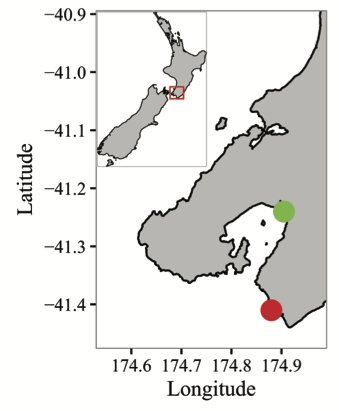
\includegraphics{images/nz_map.png}
\caption{\label{fig:nzmap}Sampling locations for juvenile G. maculatus.
Green = Hutt River. Red = Wainuiomata River. River mouths are
approximately 20 km apart. Data for the maps comes from the `maps'
(Becker et al. 2016) and `mapdata' (Becker et al. 2016) R packages.}
\end{figure}

\subsection{Statistical Analysis}\label{statistical-analysis}

To evaluate spatio-temporal variation in G. maculatus developmental
characteristics I fit three nested linear models (using standard length,
average growth rate, and age as response variables in three separate
models). Predictor variables included in each model were \emph{site}
(Hutt and Wainuiomata), \emph{month} (4 months in the Hutt, 3 in the
Wainuiomata), and \emph{day} (4 days per month for each site). I
included main effects of site, month, and day, and the interaction term
of site x month. The day effect was nested within the interaction term
as I only wanted to compare days that occurred within the same month and
site. I hypothesized that all three response variables would show
different patterns across months given divergent dispersal patterns and
associated environmental conditions experienced. I did not expect to see
any differences across days or between sites as I assumed larvae would
all have experienced similar environmental conditions (or similar enough
that differences would not be detectable). Therefore, I treated all
terms in the model as fixed effects so I could specifically evaluate the
differences between the levels of each factor. I conducted post hoc
tests, using the `lsmeans' procedure from the `lsmeans' package (Lenth
2016), to evaluate 4 aspects of each model: Do developmental
characteristics (1) vary between sites (main effect: site); and (2) vary
across months (main effect: month). (3) Does the pattern of variation
between sites differ across months (interaction: month x site). (4)
Using the nested term I also evaluated variation in developmental
characteristics across days within sites and months (nested main effect:
day). When there was a significant interaction, I ran post hoc tests to
evaluate aspects (1) and (2), see above. If there was no significant
interaction, post hoc tests were run on each main effect.

\section{Results}\label{results}

I evaluated spatial and temporal variation in developmental
characteristics with a sample of 496 fish. Standard length ranged from
33.7 to 51.2mm (mean = 45.5, SD = 2.3). Ages ranged from 105 to 233 days
(mean = 175, SD = 18.5). Otolith growth rates ranged from 1.27 to 2.25
μm-1day-1 (mean = 1.67, SD = 0.163).

\subsection{Spatio-temporal variation in standard
length}\label{spatio-temporal-variation-in-standard-length}

I found a non-significant effect of the interaction term (F2, 470 =
1.95, p = 0.144, \ref{fig:anova1}) suggesting that patterns of variation
in length across months were similar between sites. Therefore I
evaluated main effects. Fish from the Wainuiomata River were longer than
fish from the Hutt River (main effect of site variable, F1, 470 = 10.74,
p = 0.001, \ref{fig:stdlengthsite}).

\begin{figure}
\centering
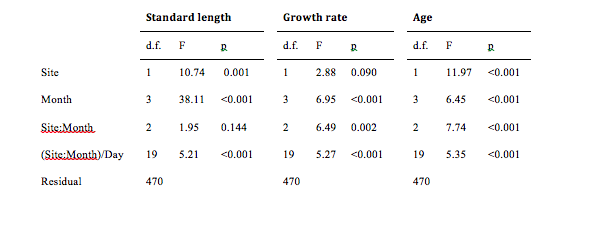
\includegraphics{images/anova_table1.png}
\caption{\label{fig:anova1}Spatio-temporal variation in length, growth rate,
and age of juvenile G. maculatus. ``Site:Month'' represents the
interaction term, and ``(Site:Month)/Day'' represents the day term,
nested within the month and site interaction term.}
\end{figure}

\begin{figure}
\centering
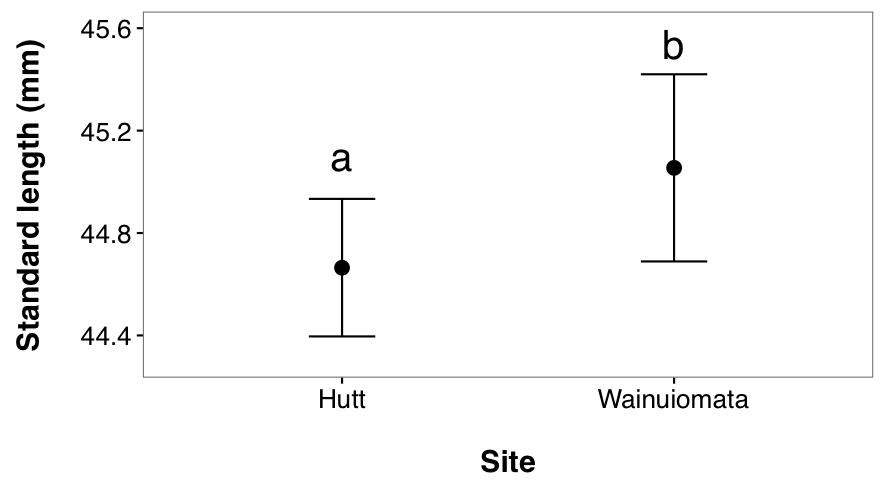
\includegraphics{images/std_length_fig1.png}
\caption{\label{fig:stdlengthsite}Spatial variation in standard length of
juvenile G. maculatus collected from two sites (Hutt River and
Wainuiomata River). Given are L-S means (i.e.~corrected for other
sources of variation in the statistical model, see table 2-1) ± 95\% CI.
Dissimilar lowercase letters indicate a significant difference based
upon post hoc tests.}
\end{figure}

Length also varied across months (main effect of month variable, F3, 470
= 38.11, p \textless{} 0.001, \ref{fig:stdlengthmonth}). A post hoc test
revealed that fish caught in August were significantly larger than fish
from September (p \textless{} 0.0001), October (p = 0.0026), and
November (p \textless{} 0.0001). Fish from September and October were
both significantly larger than November fish (p \textless{} 0.0001 for
both) but not different from one another (p = 0.4505).

\begin{figure}
\centering
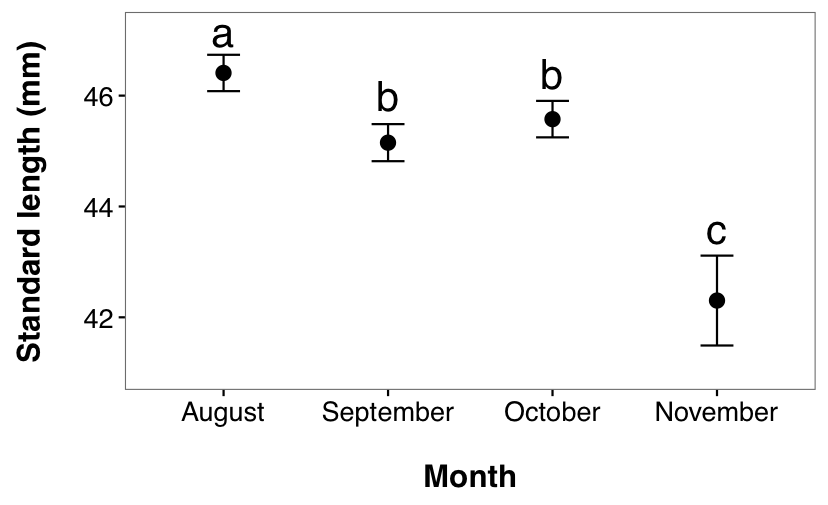
\includegraphics{images/stdlengthmonth.png}
\caption{\label{fig:stdlengthmonth}Temporal variation in standard length of
juvenile G. maculatus collected from two sites. Given are LS means ±
95\% CI. Dissimilar lowercase letters indicate a significant difference
based upon post hoc tests.}
\end{figure}

The standard length of G. maculatus varied significantly among days
nested within sites (F19, 470 = 5.210, p \textless{} 0.0001,
\ref{fig:spatiotemp1}). A post hoc test (\ref{fig:spatiotemp1table})
indicates that a small number of pairwise comparisons appear to be
driving the significance of this effect. \ref{fig:spatiotemp1} suggests
that sizes of G. maculatus are heterogeneous across consecutive days
within some months (i.e.~October, November) for the Hutt River in
particular.

\begin{figure}
\centering
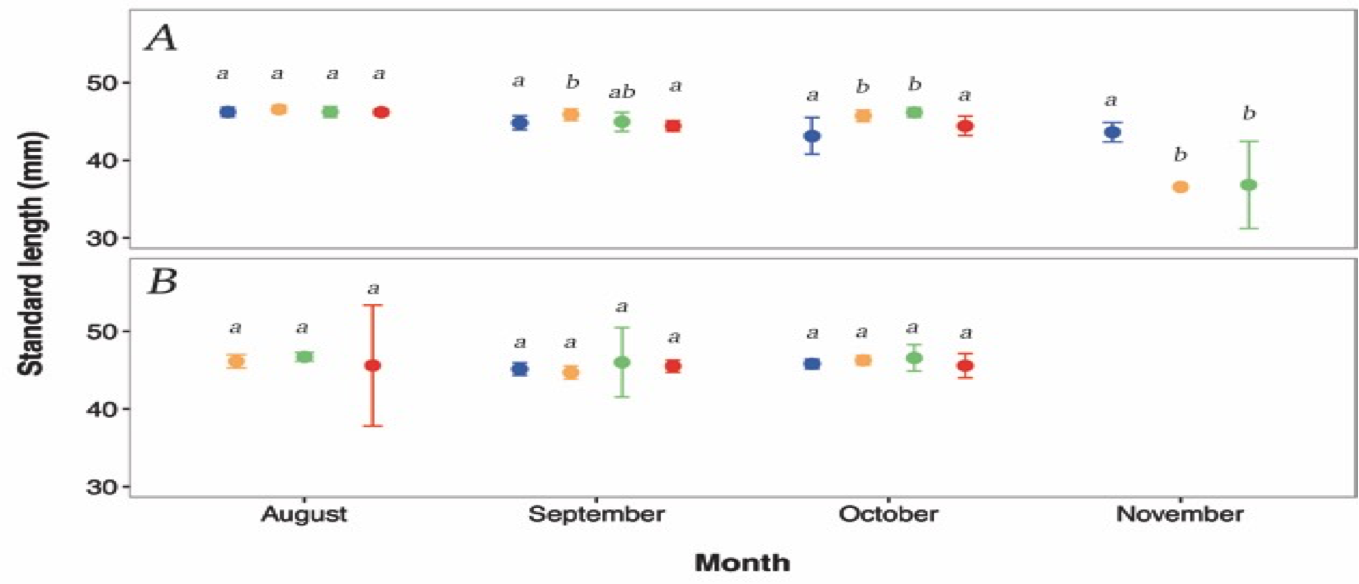
\includegraphics{images/spatiotemp1.png}
\caption{\label{fig:spatiotemp1}Daily (within month) temporal variation in
standard length between (A) Hutt River, and (B) Wainuiomata River. Given
are LS means ± 95\% CI. Different colours represent the different
sampling days. Blue=day 1, orange=day 2, green=day 3, red=day 4. Missing
symbols indicate days were no fish were sampled. Confidence intervals
are obscured by size of symbols for several observations. Dissimilar
lowercase letters indicate a significant difference based upon post hoc
tests; separate analyses were conducted for each site and month}
\end{figure}

\begin{figure}
\centering
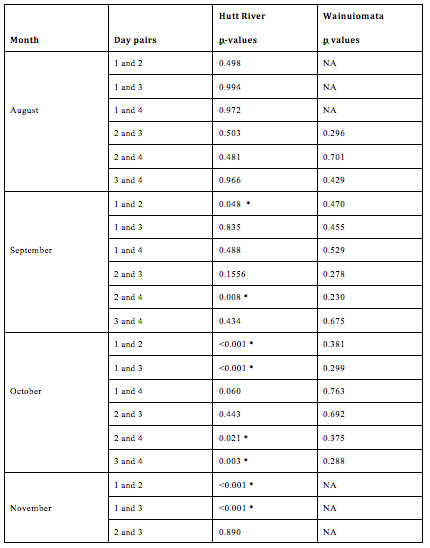
\includegraphics{images/spatiotemp1table.png}
\caption{\label{fig:spatiotemp1table}Pairwise comparisons of standard length
between days nested within months and sites. No fishing was conducted in
the Wainuiomata during November due to river mouth closure. No fish were
successfully caught on the 1st day in August in the Wainuiomata or the
4th day in November in the Hutt (as indicated by ``NA''). Asterisks
indicate a significant difference in length between day pairs.}
\end{figure}

\subsection{Spatio-temporal Variation in Average Growth
Rate}\label{spatio-temporal-variation-in-average-growth-rate}

I found a significant interaction between month and site (F2, 470 =
6.489, p = 0.0017, \ref{fig:spatiotemporalgrowthrate}), indicating that
growth rate changes over time and sites (\ref{fig:anova1}). A post hoc
test showed that, in the Hutt River, fish caught in August grew faster
than fish caught in September (p \textless{} 0.0001), October (p =
0.0265) and November (p = 0.0134). September did not differ to October
(p = 0.3105) or November (p \textgreater{} 0.9999). October and November
also did not differ (p = 0.6749). In the Wainuiomata River, August fish
did not have a significantly different growth rate to fish caught in
September (p \textgreater{} 0.9999) or October (p = 0.3072). Fish from
September and October also did not differ significantly (p = 0.5708).

\begin{figure}
\centering
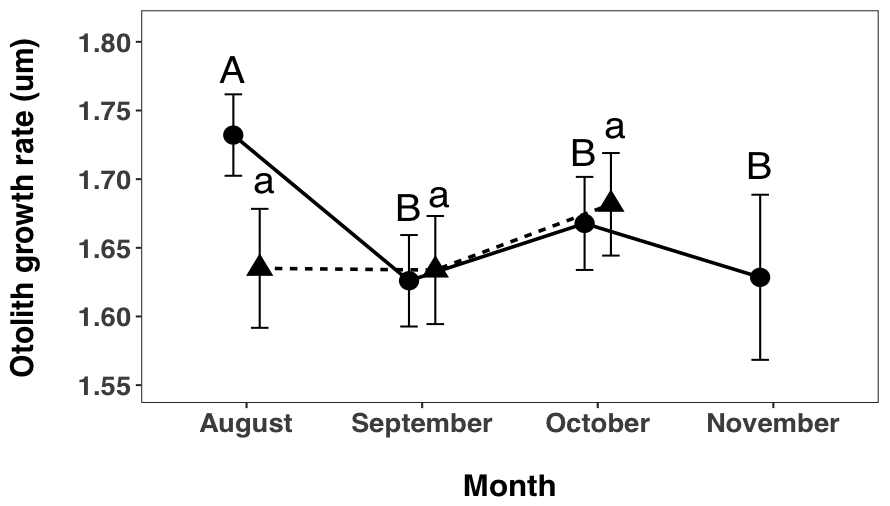
\includegraphics{images/spatiotemporalgrowthrate.png}
\caption{\label{fig:spatiotemporalgrowthrate}Spatial and temporal variation
in otolith growth rate of juvenile G. maculatus collected from two sites
(circles/uppercase letters: Hutt River, triangles/lowercase letters:
Wainuiomata River). Given are LS-means (i.e.~corrected for other sources
of variation in the statistical model (Table 2-1) ± 95\% CI. Dissimilar
letters indicate a significant difference within sites, across time
(e.g., no difference across months within the Wainuiomata River).
Sampling did not occur in the Wainuiomata River during November due to
river mouth closure.}
\end{figure}

The otolith growth rate varied significantly among days nested within
months and sites (F19, 470 = 5.2703, p \textless{} 0.0001,
\ref{fig:growthratebyday}). A post hoc test (Table 2 3) indicates that a
small number of pairwise comparisons are driving the significance of
this effect. \ref{fig:growthratebyday} suggests that otolith growth
rates of G. maculatus are heterogeneous across days within all months
for the Hutt River and homogenous across days within all months for the
Wainuiomata River.

\begin{figure}
\centering
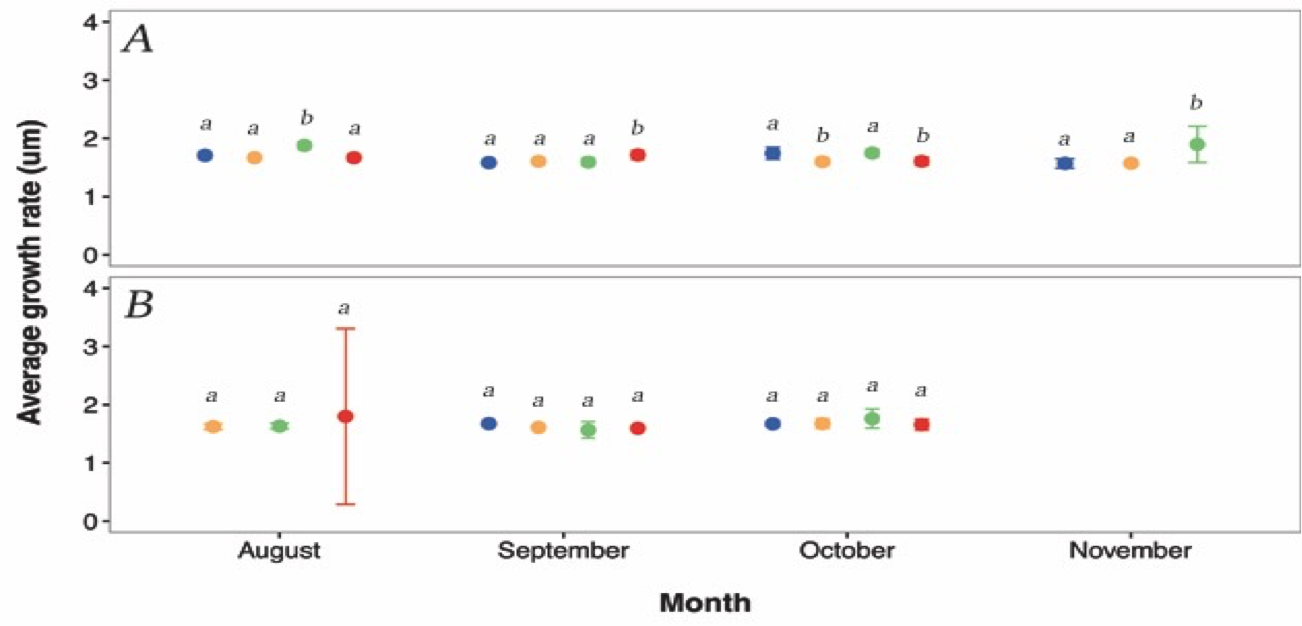
\includegraphics{images/growthratebyday.png}
\caption{\label{fig:growthratebyday}The otolith growth rate varied
significantly among days nested within months and sites (F19, 470 =
5.2703, p \textless{} 0.0001, Figure 2 6). A post hoc test (Table 2 3)
indicates that a small number of pairwise comparisons are driving the
significance of this effect. Figure 2 6 suggests that otolith growth
rates of G. maculatus are heterogeneous across days within all months
for the Hutt River and homogenous across days within all months for the
Wainuiomata River.}
\end{figure}

\begin{figure}
\centering
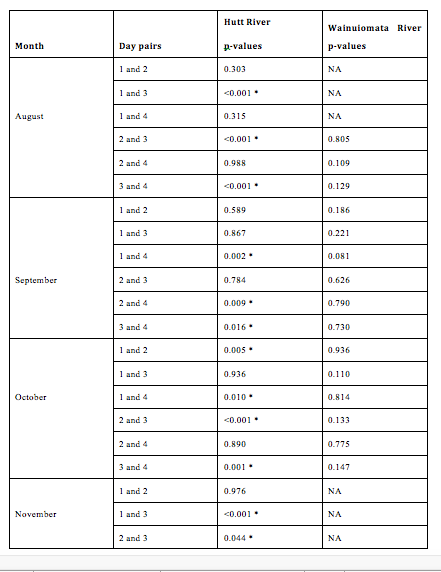
\includegraphics{images/spatiotemp2table.png}
\caption{\label{fig:spatiotemptable2}Pairwise comparisons of average otolith
growth rate between days nested within months and sites. No fishing was
conducted in the Wainuiomata during November due to river mouth closure.
No fish were successfully caught on the 1st day in August in the
Wainuiomata or the 4th day in November in the Hutt (as indicated by
``NA''). Asterisks indicate a significant difference in length between
day pairs.}
\end{figure}

\subsection{Spatio-temporal Variation in
Ages}\label{spatio-temporal-variation-in-ages}

I found a significant interaction between month and site (F2, 470 =
7.7421, p = 0.0004, \ref{fig:spatiotemporalage}), indicating that
patterns of age variation changed across time and sites. A post hoc test
showed that, in the Hutt River, fish caught in August were significantly
younger than fish caught in September (p \textless{} 0.0001), and
October (p = 0.0029) but not November (p = 0.3783). Fish caught in
September did not differ to fish from October (p = 0.4134) or November
(p = 0.2774). There was also no difference in fish caught from October
and November (p = 0.8869). In the Wainuiomata River, fish caught in
August showed no difference in age to fish caught in September (p =
0.9934) or October (p = 0.7513). Fish caught in September also showed no
difference to fish caught in October (p = 0.8709).

\begin{figure}
\centering
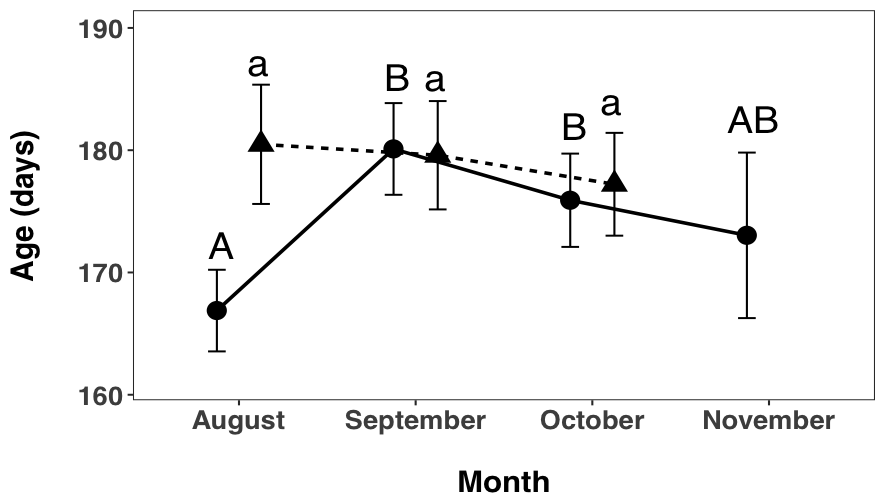
\includegraphics{images/spatiotemporalage.png}
\caption{\label{fig:spatiotemporalage}I found a significant interaction
between month and site (F2, 470 = 7.7421, p = 0.0004, Figure 2 7),
indicating that patterns of age variation changed across time and sites.
A post hoc test showed that, in the Hutt River, fish caught in August
were significantly younger than fish caught in September (p \textless{}
0.0001), and October (p = 0.0029) but not November (p = 0.3783). Fish
caught in September did not differ to fish from October (p = 0.4134) or
November (p = 0.2774). There was also no difference in fish caught from
October and November (p = 0.8869). In the Wainuiomata River, fish caught
in August showed no difference in age to fish caught in September (p =
0.9934) or October (p = 0.7513). Fish caught in September also showed no
difference to fish caught in October (p = 0.8709).}
\end{figure}

The ages of juvenile G. maculatus differed significantly among days
nested within month and site (F19, 470 = 5.3537, p \textless{} 0.0001,
\ref{fig:spatiotemp3}). A post hoc test (\ref{fig:spatiotemp3table})
again indicates that the significance of this effect is driven by a
small number of pairwise comparisons in the Hutt River.
\ref{fig:spatiotemp3} suggests that ages of G. maculatus are
heterogeneous across days within all months for the Hutt River and
homogenous across days within all months for the Wainuiomata River.

\begin{figure}
\centering
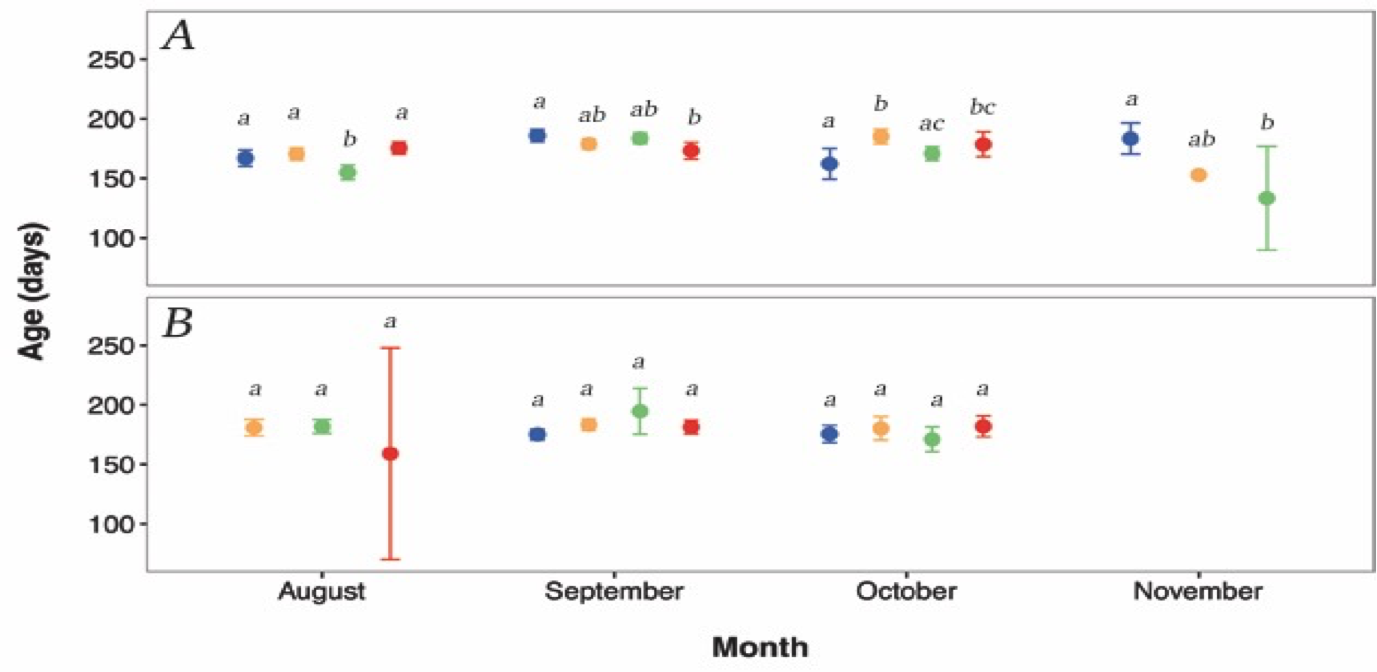
\includegraphics{images/spatiotemp3.png}
\caption{\label{fig:spatiotemp3}Daily (within month) temporal variation in
age between (A) Hutt River, and (B) Wainuiomata River. Different colours
represent the different sampling days. Blue=day 1, orange=day 2,
green=day 3, red=day 4. Missing symbols indicate days were no fish were
sampled. Error bars represent 95\% confidence intervals. Confidence
intervals are obscured by size of symbols for several observations.
Dissimilar lowercase letters indicate a significant difference based
upon post hoc tests; separate analyses were conducted for each site and
month. Sampling did not occur in the Wainuiomata River during November
due to river mouth closure.}
\end{figure}

\begin{figure}
\centering
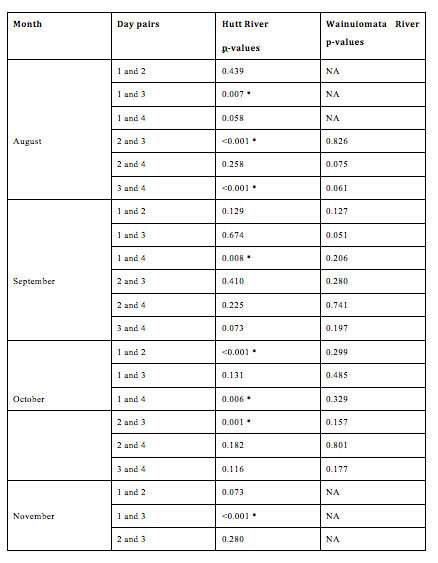
\includegraphics{images/spatiotemp3table.png}
\caption{\label{fig:spatiotemp3table}Pairwise comparisons of average growth
rate between days nested within months and sites. No fishing was
conducted in the Wainuiomata during November due to river mouth closure.
No fish were successfully caught on the 1st day in August in the
Wainuiomata or the 4th day in November in the Hutt. Asterisks indicate a
significant difference in length between a pair of days.}
\end{figure}

\section{Discussion}\label{discussion}

\subsection{Summary of Results}\label{summary-of-results}

I found site-specific trends in the developmental histories of G.
maculatus. Juvenile G. maculatus entering the Wainuiomata River showed
no difference in growth rate or age across months, although they did
show a decrease in standard length across months. Fish from the Hutt
River also shared this decrease in standard length, but also showed a
decrease in otolith growth rate. Age showed a hump shaped curve, where
the youngest recruiting fish were in August and November. Fish in the
Hutt River during August, were the youngest, fastest growing, and
largest, a pattern that was not reflected in the Wainuiomata. However,
while fish from the Wainuiomata River did not show significant
differences in otolith growth rate and age, there did appear to be
non-significant trends that matched the results from the Hutt River.

There was no day-to-day variation in any developmental characteristics
of fish sampled from the Wainuiomata River. While fish from the Hutt
River did show day-to-day variation, there was significant variation in
the direction and magnitude of trends. Therefore, the two main points of
interest become (1) why was there daily and monthly variation through
time, and (2) why was there more variation in the Hutt River?

\subsection{Spatial Differences in Developmental
Histories}\label{spatial-differences-in-developmental-histories}

I propose two hypotheses that could explain my results (and these are
not mutually exlusive): (1) the Hutt River may be replenished by fish
from a wider variety of source populations than the Wainuiomata River,
which could lead to greater variation in developmental histories among
cohorts (natal source hypothesis), and/or (2) recruits from the Hutt
River may have experienced greater environmental variability during
their pelagic larval dispersal phase, which could lead to different
phenotypic distributions through individual fish experiencing phenotypic
plasticity or selective mortality (environmental experience hypothesis).

A difference in the composition of source populations entering each
river is dependent on the extent of dispersal. G. maculatus have very
strong swimming capabilities (Barker and Lambert 1988), and considerable
research has examined the extent of population mixing and natal return
(Barker and Lambert 1988, Berra et al. 1996, Waters and Burridge 1999,
Waters et al. 2000) with current paradigms suggesting that G. maculatus
does not show extensive natal homing (Waters et al. 2000, Hickford and
Schiel 2016). However most evidence is based off a lack of genetic
structure among sampled populations, and genetic structuring may be
mediated by only a small number of mixing individuals (Hartl 1988).
Furthermore, most studies have been concerned with broad spatial
hypotheses (Barriga et al. 2007, Barbee et al. 2011, Barriga et al.
2012), rather than considering the characteristics of individual systems
that may facilitate a higher level of retention than the majority of
source populations. Harbour systems have been shown to have highly
retentive properties due to physical and hydrodynamic processes acting
on the water currents (Maxwell 1956, Bowman et al. 1983, Anderson 1988).
Therefore I suggest that the hydrodynamic characteristics of the
Wellington Harbour may promote higher retention of larval G. maculatus
than would be expected by a coastally positioned system, thus promoting
self recruitment (Jones et al. 2005, Levin 2006, McDowall 2009).
However, I do not assume that the Wellington Harbour is completely
isolated from other (perhaps coastally derived) G. maculatus
populations, and I would expect it to still receive input from other
source populations around New Zealand (McDowall et al. 1975, Caley et
al. 1996, McDowall 2002, Swearer et al. 2002). The combined input of
recruits from other source populations (with their own variations in
phenotype), plus the resident population in the Wellington Harbour, may
combine to produce a more heterogeneous population of G. maculatus
(Shima and Swearer 2009). Fish from the Wellington Harbour would
therefore show a wider distribution in phenotypes than the Wainuiomata
River, which may not have a resident population, and is only replenished
by regional source populations (that shared more similar environmental
conditions). These differences in the spread of potential phenotypes may
be driving the lack of significant differences in the Wainuiomata, while
accounting for the range of patterns documented in the Hutt River.

Marine habitats can show considerable variation in temperature, water
flow, light availability, and salinity (Johnston 2006) which may vary
extensively through time. Pelagic fish may experience phenotypic
plasticity as a result of this environmental variability, and therefore
their phenotype may correlate with conditions experienced during
dispersal. If my two study sites are replenished by different
combinations of source populations, with differing dispersal histories,
then the environmental conditions experienced may be driving these site
specific differences. During dispersal, cohorts may encounter novel
environments that impose directional selection on phenotypic traits
(Reznick and Ghalambor 2001, Grether 2005), which shifts the mean
phenotype to a new peak (Lande and Arnold 1983). Environmental pressures
may be either biotic (Handelsman et al. 2013) or abiotic (Carrera et al.
2012) but all have the potential to drive phenotypic shifts (Agrawal
2001). This hypothesis is dependent upon Wellington Harbour showing a
higher degree of temporal variability in its biotic and abiotic
conditions. Under the assumption that it is more variable, individuals
with recent resident periods in the harbour may have experienced
phenotypic plasticity, and therefore developed phenotypic
characteristics representative of the conditions at the time (Agrawal
2001, Barriga et al. 2012, Chapman et al. 2015). Depending on the scale
of this variability it may account for both monthly and daily
differences. In contrast, if the Cook Strait shows a less temporally
variable environment then that may explain the fairly consistent trends
in phenotypes of recruits.

General trends in harbour systems have shown evidence of circulation
currents leading to high levels of nutrients (Mackas and Harrison 1997)
and zooplankton (Soetaert and Herman 1994). They have also shown that
abiotic conditions can be highly variable between seasons (Muylaert and
Raine 1999). Results by Maxwell (1956) indicate average water
temperatures in the Wellington Harbour increase from August to November,
yet there is also considerable fluctuation over shorter time scales,
with changes of up to 2.5°C within a three day period. Maxwell (1956)
also postulated that the causes of this high variability was due to the
sheltered positioning of the harbour. In contrast, Cook Strait has very
high energy, fast flowing currents (Bowman et al. 1983), and its lack of
shelter may not promote high levels of abiotic variability. Cook Strait
is highly dynamic with complex patterns of water circulation, but there
is little evidence for its low productivity waters being temporally
variable (Bowman et al 1983). While it may be a high energy environment,
I argue that the consistent nature of it is not enough to drive
phenotypic differences in resident cohorts of G. maculatus.

\chapter{\texorpdfstring{Implications of Variable Larval Quality on
Juvenile Mortality in \emph{Galaxias
Maculatus}}{Implications of Variable Larval Quality on Juvenile Mortality in Galaxias Maculatus}}\label{implications-of-variable-larval-quality-on-juvenile-mortality-in-galaxias-maculatus}

\section{Introduction}\label{introduction-2}

Marine organisms with stage structured life histories can experience
very high mortality rates during their planktonic phase (Hjort 1914,
Bailey and Houde 1989). This level of mortality can be mediated by
growth rates, where selective mortality favours individuals with
specific patterns of growth (Anderson 1988). Fast growth may be
beneficial if it enables fish to outgrow gape limitations of predators
(Hambright 1991), improve upon their swimming ability to escape
predators (Litvak and Leggett 1992), and/or store sufficient energy to
avoid starvation (Shuter et al. 1980, Conover and Schultz 1997).
Conversely, slow growth can be beneficial if fish become more
inconspicuous to predators (Biro et al. 2004) or undertake behavioural
changes to minimise their vulnerability (Meekan et al. 2010)

An individual's growth rate may be correlated with its rearing
environment. Biotic and abiotic factors may influence the magnitude of
growth rate, resulting in phenotypes being partially influenced by
developmental environment (Agrawal 2001). Environmental variables known
to influence growth rate include temperature (Green and Fisher 2004),
presence of predators (Milano et al. 2006), water movement (Kekalainen
et al. 2010), and food availability (Jones 1986), although relationships
may be positive, negative, and/or non-linear. Optimal temperatures and
food availability will usually promote higher levels of growth
(MacDonald and Thompson 1985) although these relationships can be
complex and context dependent (Nicieza and Metcalfe 1997). A substantial
body of evidence indicates that growth is also linked with fitness
(Cowan et al. 1996, Searcy and Sponaugle 2001, Shima and Findlay 2002,
Raventós and Macpherson 2005, Grorud-Colvert and Sponaugle 2006, Shima
and Swearer 2009), with further evidence indicating that increases in
fitness may be linked with growth in early life (Shima and Findlay 2002,
Gagliano et al. 2007), and growth immediately preceding life stage
transitions (Hamilton 2008, Hamilton et al. 2008). In species with
protracted spawning and a pelagic dispersal phase, separate cohorts of
fish may experience different conditions due to natural temporal
variation in the environment (i.e.~across seasons). Long distance
dispersal can be a physiologically demanding event, and often results in
high levels of mortality (Baker and Rao 2004).

There are well defined conceptual frameworks for the relationship
between growth and mortality (Anderson 1988). The growth-mortality
hypothesis (Ware 1975, Shepherd and Cushing 1980) generally predicts
that growth will be related to mortality, typically through the
mechanisms of starvation and/or predation. However, both of these
processes typically elucidate different relationships between growth and
mortality (Anderson 1988, Leggett and Deblois 1994). Limitation by food
can lead to a relationship where fish with higher growth rates
experience lower mortality. Prey can often be distributed non-uniformly,
and it has been suggested that ambient prey density in the ocean is too
low to support growth and survival of larval fish (Anderson 1988).
Larger larvae are less susceptible to starvation than smaller
conspecifics, due to having excess fat reserves (Hjort 1914), and
therefore are more likely to survive intense periods of starvation
(i.e., over winter mortality). Growth and mortality would therefore show
an inverse relationship, where fish with higher growth rates would
experience lower levels of mortality.

Limitation by predators can show a different relationship, where prey
mortality follows a dome shaped curve. Under this model, fish with the
highest and lowest growth rates will experience the highest levels of
mortality. Fish are the most significant predators of fish larvae (Pepin
1987, Bailey and Houde 1989) and they are known to cause significant
levels of mortality (Ware 1975, Sissenwine 1984, Gaines and Roughgarden
1987, Bailey and Houde 1989). Predation by fish requires larvae to be
encountered, attacked, and captured (Pepin 1992). Small fish with have a
low encounter rate, but a high capture rate, whereas large fish will
have a high encounter rate with a low capture rate, thus producing the
relationship where intermediate sizes convey the highest fitness
(Leggett and Deblois 1994).

Here, I examine how mortality varies as a function of larval quality in
an amphidromous fish (Galaxias maculatus) during a migratory phase in
its life cycle. Adult G. maculatus are primarily semelparous (McDowall
1968, but see Stevens et al 2016). Across a population, however,
spawning occurs over a period of several months. Larvae spend 3-6 months
developing in the open ocean before migrating (as metamorphosed
juveniles) to freshwater streams, where they develop for a further
\textasciitilde{}six months before spawning (McDowall 1990). In New
Zealand, upstream migration occurs year round, however migration peaks
from August to November (McDowall et al. 1994). Environmental conditions
(e.g.~temperature, food availability) vary over the recruitment period,
setting up an expectation for temporal variation in the quality of
incoming recruits. I build on my results from chapter 2 by exploring the
relationship between phenotypic `quality' and mortality rates.
Specifically, I used the same samples of fish from the methodology in
chapter 2 and used otolith based reconstructions of fish life histories
to derive a measure of larval quality. I quantified the mortality rates
experienced by each daily cohort, and investigated whether these two
traits were interrelated. As larval fish are susceptible to both
starvation and predators, I hypothesised that the relationship between
mortality and larval quality would follow either the linear,
food-limited trend, or the dome-shaped, predation-limited trend.

\section{Methods}\label{methods-1}

\subsection{Fish collections}\label{fish-collections-1}

Briefly, I sampled incoming G. maculatus recruits from two rivers in the
Wellington area. Sampling was conducted so that fish were collected
across the main recruitment season (August to November). For a full
description of juvenile sampling, see chapter 2.

\subsection{Characterising larval
quality}\label{characterising-larval-quality}

Following the general approach of Shima and Swearer (2009), I used the
daily otolith increments to estimate four variables that describe the
phenotypic `quality' of incoming G. maculatus recruits: (1) ``Pelagic
larval duration'' (PLD) is an estimate of the time the individual has
spent developing as a larvae, and was estimated as the number of daily
rings. (2) ``Average growth rate'' is a measure of the average amount of
somatic growth an individual experienced on a given day, and was
estimated as the average distance between successive daily rings. (3)
``Early growth rate'' was estimated as the average distance between the
first 20 daily rings. (4) ``Late growth rate'' was estimated as the
average distance between the last 20 daily rings.

I centered and scaled the four variables (mean = 0, SD = 1) and
performed a principal components analysis, using the `prcomp' function
in RStudio v0.99.903 (RStudio Team 2015) , to derive a composite metric
of `larval quality' score (i.e., first principal component).

\subsection{Estimating mortality
rates}\label{estimating-mortality-rates}

To estimate mortality rates I used the Chapman-Robson approach to
catch-curve analysis (Chapman and Robson 1960, Robson and Chapman 1961).
Catch curve analysis is used to estimate mortality by measuring the
decline of the number of individuals in the age classes of a cohort
(Pauly 1990). Traditional catch-curve analysis (Ricker 1975) would fit a
linear regression to the descending limb of an age-frequency curve,
under the assumption that the ascending limb of the curve contains fish
too young to recruit to the fishery or gear. The Chapman-Robson method
instead treats the descending limb of the curve as following a geometric
probability distribution, and computes a maximum likelihood estimator
for annual survival (Chapman and Robson 1960, Robson and Chapman 1961).
Instantaneous mortality rates (Z) can then be computed using
Z=-log(annual mortality), however these estimates have be shown to be
slightly biased, so I instead used the correction offered by Hoeing et
al (1983). The Chapman-Robson approach was chosen over more traditional
methods due to the findings of Dunn et al (2002) and Smith et al (2012)
who showed that this method is the most precise, and produces the least
variance. All calculation of Z scores was done with the `FSA' package
(Ogle 2016) in RStudio v0.99.903 (RStudio Team 2015).

\subsection{Evaluating the relationship between mortality and
quality}\label{evaluating-the-relationship-between-mortality-and-quality}

For this analysis, I assumed that samples collected on different days
were independent of one another (i.e.~I did not model the temporal
structure of my sampling design; c.f. Chapter 2). For each sample day at
each site I computed average larval quality and instantaneous mortality
rate (i.e., estimated for fish collected from a given site on the same
day). Because preliminary analysis (loess regression) indicated a linear
relationship between instantaneous mortality and larval quality, I used
a linear model for my formal analysis. Specifically, I used an ANCOVA
model to evaluate the relationship between instantaneous mortality (the
response variable) and larval quality (the covariate), and whether the
intercept and/or the slope of this relationship varied between sites.

\section{Results}\label{results-1}

The first principal component accounted for 54\% of the variation in the
larval quality variables. PLD loaded positively on PC1, while the three
growth variables all loaded negatively. Fish with higher PC1 scores
therefore had long PLDs with slow growth. Since a low PC1 score would
indicate a fish of higher `quality' (i.e., faster growth and development
time), I multiplied all PC1 scores by -1 for purposes of presentation
(i.e.~so that the re-expressed PC1 scores scale more intuitively with
traits often associated with `larval quality'.

\subsection{Relationship between mortality and larval
quality}\label{relationship-between-mortality-and-larval-quality}

The relationship between instantaneous mortality rate and average larval
quality was consistent across sites (interaction term: F1,17 = 1.3262, p
= 0.2654). Therefore I evaluated a reduced model using only main effects
of larval quality and site. Instantaneous mortality rates did differ
between sites (F1,18¬ = 0.0891, p = 0.7688), and there was no
significant relationship between instantaneous mortality rates and
larval quality (F1,18 = 3.2712, p = 0.0872). Although the model was not
significant, there does appear to be a trend towards higher quality fish
experiencing lower mortality (\ref{fig:mortality-rates}). The power of
the model was very low (0.2751) based off detecting a `medium' effect
size, so non-significance may be attributable to insufficient sample
size. Power analysis indicated that a sample of \textasciitilde{}60
would give the model a more reasonable power of 0.8.

\begin{figure}
\centering
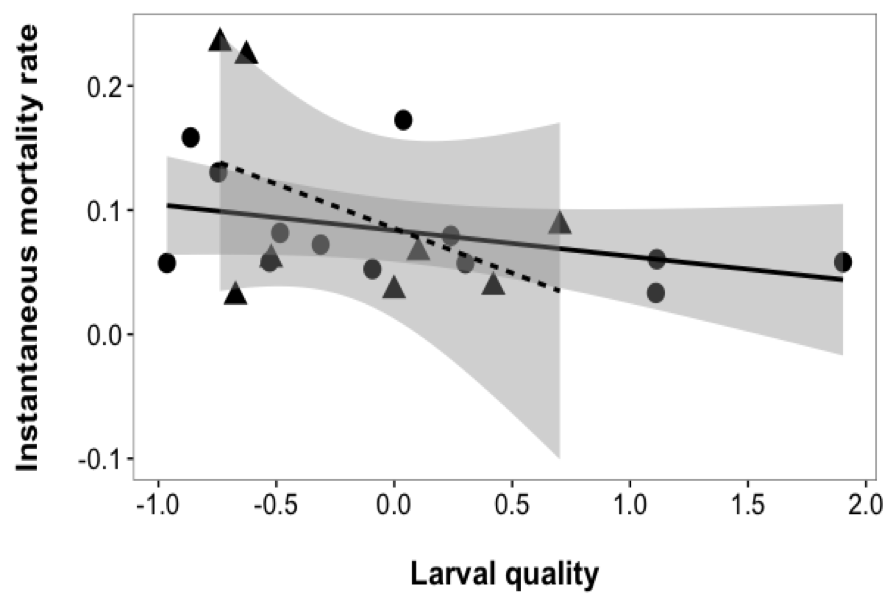
\includegraphics{images/data-chapter-2/mortality-rates.png}
\caption{\label{fig:mortality-rates}Relationship between instantaneous
mortality rate (Z score) and average larval quality (PC1) for each daily
cohort of G. maculatus from two sites: circle/solid line = Hutt River,
triangle/dashed line = Wainuiomata River. Shaded lines represent the
95\% confidence interval around the regression lines.}
\end{figure}

\section{Discussion}\label{discussion-1}

Few studies have addressed threats during the marine phase of the G.
maculatus life cycle (Barriga et al. 2007, Jellyman and McIntosh 2008).
Fish undertaking dispersal in the open ocean can be subject to
environmental factors, such as temperature (Pepin 1991) and food (Einum
2003) fluctuations, that may cause changes in growth rate. Understanding
changes in growth, and how it relates to mortality rates, may provide
information on factors that constrain fish populations during dispersal.
Growth-mortality relationships are often non-linear (e.g.~U-shaped),
where highest mortality is experienced by the fastest and slowest
growers (Anderson 1988, Staudinger and Juanes 2010), or negatively
linear, where highest mortality is experienced by the slowest growers
(Leggett and Deblois 1994). However, my results did not appear to follow
either of these trends.

Phenotype is at least partially influenced by environment (Meekan et al.
2003, Sponaugle et al. 2006), and cohorts of G. maculatus with varying
dispersal pathways may show evidence of this through their phenotype. My
previous chapter demonstrated site specific differences in growth rates,
yet here site was unrelated to differences in mortality rates. These
results suggest that mortality is not a function of dispersal pathway
(assuming different phenotypes from Chapter 2 would result in different
mortality rates), and is experienced consistently across spatial scales.
While environmental variation may be strong enough to significantly
differentiate phenotypes between spatially separated cohorts, it may not
cause differing levels of mortality in larval G. maculatus. While G.
maculatus are known to have high levels of phenotypic plasticity
(Barriga et al. 2002), it appears that factors governing mortality are
either unrelated to phenotype, or they are shared, both in direction and
magnitude, producing similar larval quality distributions.

Instantaneous mortality rate also appeared to be unrelated with larval
quality. My results did show a weak negative trend, which would be a
characteristic of food limitation, however this trend was
non-significant. The model used to evaluate this relationship had very
low power (0.2751), which may have constrained its ability to detect a
significant relationship, however my results seem to suggest that a
factor other than food or predators is causing mortality in cohorts of
G. maculatus. While starvation and predation are some of the strongest
forces affecting larval survival (Leggett and Deblois 1994), it is
important to consider that there are multiple sources of mortality that
affect larvae (Pineda et al. 2009). Specifically, catch-curve analyses
do not consider mortality due to advection, and transport away from
suitable settlement habitat (White et al. 2014). Therefore, an
alternative interpretation is that my mortality estimates have assumed
the mortality of recruits that are still alive, but were transported
away from my study areas and settled elsewhere. Thus, they are presumed
dead by the catch-curve model (due to not being sampled). Therefore,
while the study of larval transport and retention is important in
understanding phenotypic patterns (c.f. Chapter 2), it may also be
important in understanding mortality patterns.

An alternative explanation for my results is that my sampling may
reflect a population that has already experienced extensive selective
mortality. Sampled fish may only represent the survivors, and therefore
my sampling may have not captured the `larval quality' scores of fish
that experienced strong mortality pressures. Therefore, the relationship
between quality and mortality may have originally followed a more
typical U-shaped relationship (Anderson 1988) but, post-mortality, only
the centre of this spectrum remains (or some segment of this pattern).
As the more extreme edges of the growth-mortality curve may not be able
to be detected, the non-linear relationship becomes masked to this
analysis. Overcoming this limitation in future studies may be difficult,
and require extensive sampling of larval G. maculatus during their
marine dispersal phase.

This lack of mortality due to abiotic factors ties in further with my
results from Chapter 2. While not explicitly evaluated in this chapter,
fish from the Hutt River appears to have a wider range of larval quality
scores, but a smaller range of mortality rates, than fish from the
Wainuiomata River (\ref{fig:mortality-rates}). These are similar results
to Chapter 2, where I found strong spatial differences in phenotypes
between each river. Similarly to Chapter 2, this result could indicate a
more heterogeneous rearing environment (i.e., environmental experience
hypothesis), which allows a greater scope for extreme phenotypes to
persist. Wellington Harbour may act as a `nursery' ground, where
environmental heterogeneity drives phenotypic differentiation, but also
provides more refuge from lethal effects (i.e., as seen in the lower
variability in mortality rate, \ref{fig:mortality-rates}).

Estimates of instantaneous mortality rates based upon catch-curve
analyses depend upon several important assumptions (Ricker 1975).
Specifically, it assumes that the population being tested is closed,
with no immigration or emigration, and that all age classes are equally
recruited to the fishing gear. Populations of G. maculatus are generally
considered to be demographically open (Waters et al. 2000), due to their
significant dispersal capabilities, however, other studies have used
this technique on open populations (Sandström and Thoresson 1988, Irvine
et al. 2007, Windsland 2014). The assumption of a closed population is
assuming a study system with a standing stock of individuals, of which
recruits are added to through time (Ricker 1975). G. maculatus typically
die at one year of age, and so my sampling does not reflect mortality in
a standing stock, rather, it is only considering these new recruits. In
essence, this analysis is based around a daily stock recruitment model,
rather than an annual one. Furthermore, Ricker's initial methodology was
based around using fish that were grouped into year classes rather than
day classes, and most subsequent applications of the method have used
year class fish (Hoffnagle and Timmons 1989, Restrepo et al. 2007, Kell
et al. 2013). However, the technique has been applied to day class fish
(Essig and Cole 1986) and to G. maculatus specifically (Barriga et al.
2012). Due to the prevalence of this technique, and that I am only
treating each daily cohort as a closed population, I believe that my
results are robust enough to be interpreted with caution. While I do not
claim they represent a `true' measure of mortality, they are still
useful to draw inference from.

This study has demonstrated that there appears to be little relationship
with the quality of recruiting G. maculatus and their relative mortality
rates. There did appear to be a trend towards lower rates of mortality
when fish were higher quality, but this may require higher sample sizes
and longitudinal sampling of a cohort to validate. These results suggest
that understanding dispersal may be a critical factor in studies of
mortality, and that sources of mortality may operate indiscriminately on
phenotypically different populations. They also suggest that a
`phenotypically' superior G. maculatus individual may not experience
lower mortality, and have therefore have implications for the carry-over
effects that individuals may experience post-settlement.

\chapter{\texorpdfstring{Adult \emph{Galaxias Maculatus} Recruitment is
Shaped by Juvenile Growth and Hatch
Date}{Adult Galaxias Maculatus Recruitment is Shaped by Juvenile Growth and Hatch Date}}\label{adult-galaxias-maculatus-recruitment-is-shaped-by-juvenile-growth-and-hatch-date}

\section{Introduction}\label{introduction-3}

An individual's chance of surviving to successfully reproduce may be
affected by a variety of factors. Fitness may be linked to size,
condition, growth, and hatch date (Anderson 1988, Jakob et al. 1996,
Jacob et al. 2009, Buston and Elith 2011) and therefore fish may
experience selective mortality by any or all of these characteristics.
Selection on phenotypes is widely recognised across ecosystems, but the
mechanisms are often system- (Houde 1989, Kaemingk et al. 2013) and
context-dependent (Cargnelli and Gross 1996, Garvey et al. 2002).
Temporal variation in the biotic and abiotic factors of an environment
can lead to selective pressures on larval fish that vary based on an
individual's hatch date (Cargnelli and Gross 1996). Both hatch date
(Lande and Arnold 1983, Kohler et al. 1993, Cargnelli and Gross 1996,
Santucci Jr and Wahl 2003) and growth history (Leggett and Deblois 1994,
Sogard 1997) have been linked to survivorship in fish. Selective
pressures may act on both these traits to preferentially favour fish
that have hatched at the `right time' (Garvey et al. 2002), grew at an
optimum rate (Crecco and Savoy 1985), or some combination of these two
factors. If larval fish show high phenotypic plasticity, which may offer
increased survivorship (Burgess and Marshall 2011, Burgess et al. 2012),
then the combination of phenotypic plasticity and hatching over a broad
temporal time scale may offer a population the best chance of successful
recruitment.

A substantial body of evidence indicates that hatching at the `right
time' can positively influence an individual's developmental trajectory
and future success. Early hatch dates may be beneficial due to increased
developmental time (Divino and Tonn 2007), as older and larger fish
often experience the highest survival to year one (Cargnelli and Gross
1996). Old and large fish may also be the first to spawn in a
population, and also produce the largest eggs (Simpson 1959), which
creates a feedback loop where the offspring of early spawners may be
more likely to become early spawners in the next generation. Larger fish
may also experience higher survivorship due to having excess fat
reserves to exploit in periods of starvation (Bagenal 1971). However,
while there may be ecological benefits to early hatching, potential
benefits may simply be a function of hatching at the `right time.' For
example, variation in hatch date may lead to different cohorts of larvae
experiencing different seasonal characteristics such as food
availability or temperature differences (Cushing 1969, Kohler et al.
1993, Santucci Jr and Wahl 2003, Kaemingk et al. 2013). Specific hatch
dates may increase fitness in early life stages, but subsequently
decrease fitness in later stages (Langerhans et al. 2004, Bogner et al.
2016). This variation in fitness is often linked to hatch-dependent
growth rate (Divino and Tonn 2007), where post-hatch experiences have
subsequent effects on an individual's growth rate. Earlier hatch dates
are often linked with size-dependent mortality as fish born earlier have
more time to grow and are less likely to perish (Divino and Tonn 2007).
This `bigger-is-better' hypothesis works under the assumption that a
larger fish is either too big for a predator to consume (i.e., gape
limited) and/or has the swimming ability to evade capture (Hovenkamp
1992, Meekan and Fortier 1996). However, there is also evidence of
slower growth being beneficial, as this can lead to higher levels of
predator avoidance (Amara et al. 1994, Gleason and Bengtson 1996).
Selection can operate on growth rates (Shima and Findlay 2002), and
therefore ultimately determine survivorship (Rosenberg and Haugen 1982).
In species with high variation in demographic rates, early life history
can be an indicator of rearing environment (Svanback and Eklov 2002).
Fish that have developed in warm, productive environments are more
likely to be larger, have a faster growth rate, and have more energy
reserves to dedicate to reproduction (Houde 1989). Therefore, early life
history can be used to predict future success if we know that a certain
set of traits will be beneficial for an individual at a later life stage
(Houde 1997). By sampling a population repeatedly through time it is
possible to identify changes in the distribution of phenotypes (Vigliola
et al. 2007). In species with recruitment that occurs over a period of
time, the range of recruiting phenotypes may vary through time, and
therefore the survivors among these cohorts would possess traits
necessary for future success (Cargnelli and Gross 1996).

The aim of this chapter is to understand how both hatch date and growth
rate of juvenile fish independently shape adult populations. To address
this question I sampled discrete populations of pre-settlement juveniles
throughout the peak recruitment season (McDowall et al. 1994). I sampled
the populations again six months later (post-settlement), after those
cohorts of fish had reached maturity. As fish will likely experience
different sources of mortality post-settlement and pre-settlement, I
hypothesized that mortality would be selective with respect to hatch
date and/or growth rate. Therefore, I expect to see reduced variation in
these traits when the surviving adults are sampled. Given that fish
entering the rivers early in the recruitment season have faster average
growth rates (see chapter 2) that may confer increased fitness, I
hypothesized that early hatched recruits would have increased chances of
survival. Therefore, I expected fish that entered the river in August to
comprise the majority of the adult population.

\section{Methods}\label{methods-2}

\subsection{Fish collections}\label{fish-collections-2}

I used otolith daily ring formations to characterize hatch dates and
growth histories for two life stages of the amphidromous fish Galaxias
maculatus. After hatching from eggs laid in riparian vegetation, larvae
spend approximately 6 months developing in marine areas where they have
opportunity to disperse (McDowall 1968). Fish will then migrate to, and
settle in, freshwater streams where they will spend another six months
developing into reproductively mature adults (McDowall 1968). I caught
fish from each life stage at two rivers to test whether adult fish had
similar growth histories and hatch dates to juvenile fish.

I sampled juveniles and adults from the Hutt River and the Wainuiomata
River. Juveniles were sampled over a period of months, and details of
this sampling are given in chapter 2. For analysis of growth rate I
assigned sampled fish to specific `cohorts' based upon their month of
collection. Juvenile fish were not grouped into cohorts for analysis of
hatch date.

I sampled these cohorts again approximately six months later, after the
juveniles had developed into adult fish and were ready to spawn. My
sampling regime makes the assumption that I am sampling the same set of
cohorts in each life history stage without any bias. It also assumes
that G. maculatus lives for one year and is semelparous (but see Stevens
et al. 2016). While recent evidence suggests that some individuals
survive through to year 2 and display iteroparity, the aging of all
samples would detect any year 2 fish, and therefore would not skew the
results. I sampled adult G. maculatus from spawning grounds
(i.e.~riparian vegetation covering moist riverbanks, Benzie 1968a) and
used two unbaited sock nets to catch adult fish. I only fished on days
where the high tide was ≥ 1.8 metres. The nets were set 2-3 hours before
the high tide, and were taken down approximately one hour after high
tide. The total sample size was 50 adult fish. Twenty fish were caught
from the Wainuiomata River on 19th March 2016. Thirty fish were caught
from the Hutt River over 8 separate fishing days, spread from 25th March
to 5 June 2016.

\subsection{Otolith analyses}\label{otolith-analyses}

Adult otoliths were prepared identically to the juvenile otolith
preparation described in chapter 2. Briefly, age was estimated as the
number of daily rings visible between the core and the edge of the
otolith along the postrostral axis. The complete otolith growth history
was characterised by measuring the distance between each successive ring
along the postrostral axis. I used the age of each fish to
back-calculate hatch dates of individuals. For analysis, I converted
hatch dates to a numerical `day of the year' (Julian date).

\subsection{Statistical analysis}\label{statistical-analysis-1}

I hypothesised that the sample of adult fish would show a different
hatch distribution to that of the juvenile fish sample due to selective
mortality. I also hypothesised that the sample of adult fish would show
a similar growth history to one or more of the monthly cohorts of
juveniles sampled, likely favouring faster growth. I tested each site
separately for the null hypothesis that both adult and juvenile fish
hatch dates were drawn from a common population using an
Anderson-Darling test and a one-way ANOVA test. The Anderson-Darling
test compares the shape of the hatch date distributions (Scholz and
Stephens 1987) while the ANOVA compares the mean value of the
distributions, under the assumption of a normal distribution.
Significant differences in these tests would therefore suggest the adult
population hatched at a different time to the juveniles. The
Anderson-Darling test does not have its own unique distribution (unlike
the chi-squared test). Therefore, although a test statistic and an
approximate p-value can be calculated, there is no way to calculate
critical values or degrees of freedom (Anderson and Darling 1954).
Results of the Anderson-Darling test and the ANOVA result are presented
as density plots to account for the large difference in sample sizes
between adults and juveniles.

I used a linear mixed-effects model to test whether cohorts of juvenile
fish had different otolith growth curves to the adult fish cohort. I
truncated all otolith growth data to a maximum of 180 days (the average
juvenile age) to avoid any effect of post-settlement otolith growth from
the adult fish. I modelled individual growth trajectories for each fish
(juveniles and adults) by using size-at-age of the otolith as the
response variable. Therefore, each fish had n repeated measures where n
is equal to the age of the fish, up to a maximum of 180 days. I included
a random slope and intercept for `Fish ID' to (1) allow for the
relationship between age and otolith growth to vary across individuals
and (2) allow for correlation in daily rings within each individual. I
used `age' (in days) as the continuous variable to predict the size of
the otolith. The model also included a cohort variable that accounted
for four monthly juvenile groups (August, September, October, November)
and one adult group of fish (5 levels total). The cohort variable was
included as a fixed effect to test differences in growth histories
between the adult fish and each monthly cohort of juvenile fish. I was
not interested in comparing any of the juvenile cohort's otolith growth
histories to each other: each juvenile cohort was only compared to the
adult otolith growth history, as my hypothesis was based around which
juvenile cohort(s) was similar to the adult population. This model
calculated an overall slope for each level of cohort (based on the
relationship between otolith size and age), which I interpreted as an
estimate of otolith growth rate for each cohort. I used Wald t scores to
compare the otolith growth estimate of each juvenile cohort to the
otolith growth estimate of the adult cohort. Each site was modelled
separately to facilitate these comparisons, and to account for potential
site-specific patterns (see Chapter 2). All mixed models were run using
`lme' from the `nlme' package (Pinheiro et al. 2016) in RStudio
v0.99.903 (RStudio Team 2015).

From the mixed model I obtained estimates of the otolith growth rate for
each juvenile cohort. Wald t tests were calculated in the mixed model by
setting one level of the categorical factor (the cohort variable) as a
reference level. Adult fish were set as the reference level, and so all
estimates of juvenile growth are calculated relative to the adult fish.
Therefore any juvenile cohorts that had an equal growth rate to the
adult cohort would have an estimate equal to zero.

\section{Results}\label{results-2}

\subsection{Shifts in juvenile hatch
dates}\label{shifts-in-juvenile-hatch-dates}

Results of the Anderson-Darling test suggest that the distributions of
hatch dates for adult and juvenile fish in the Hutt River did not come
from a common distribution (T = 26.09, p \textless{} 0.0001). On
average, juveniles had a hatchdate 47 days earlier than adult fish (F1,
339 = 49.602, p \textless{} 0.0001, \ref{fig:hatch-distributions}).
Adult and juvenile fish in the Wainuiomata River had hatchdates that
were drawn from a common distribution (T = 0.1761, p = 0.2937). Adult
and juvenile fish had hatchdates approximately 7 days apart, but this
difference was not significant (F1, 201 = 0.88, p = 0.3493). A density
plot represents the probability density function of a continuous random
variable (in this case, day of the year). Therefore, it allows for easy
visualisation of the two distribution curves, despite the difference in
sample sizes.

\begin{figure}
\centering
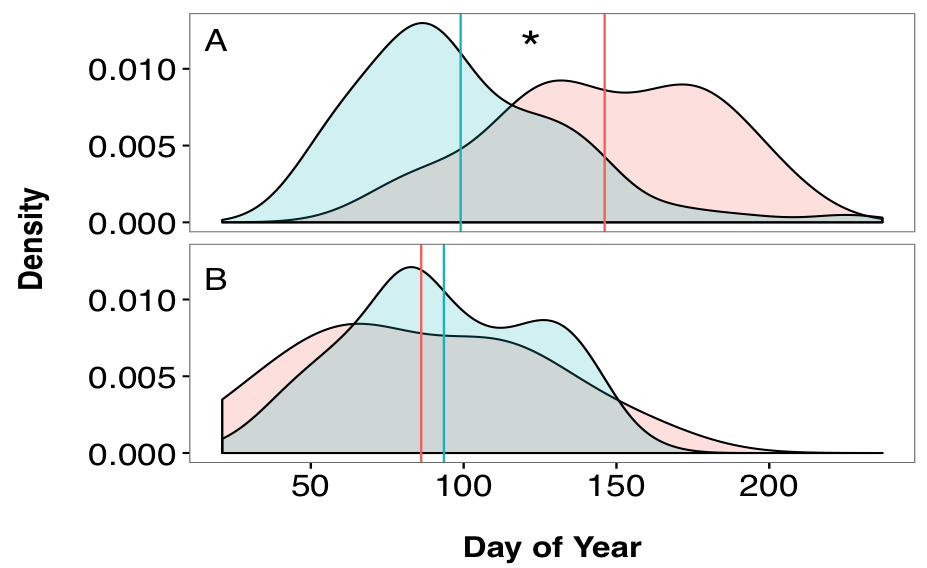
\includegraphics{images/data-chapter-3/hatch-distributions.png}
\caption{\label{fig:hatch-distributions}Comparisons of hatch date
distributions (estimated from otolith-based reconstructions) for sampled
adults (pink) and juveniles (blue) of G. maculatus. Panel (A): Hutt
River. Panel (B): Wainuiomata River. Vertical line indicates mean hatch
date for each group. Asterisk indicates dissimilar distributions and
mean values based on the Anderson-Darling test and one-way ANOVA.}
\end{figure}

\subsection{Shifts in juvenile growth
histories}\label{shifts-in-juvenile-growth-histories}

Growth histories of fish sampled from the Hutt River differed
significantly among sampled dates (i.e., among cohorts and/or between
juvenile and adult age classes; F4, 339 = 13.091, p \textless{} 0.0001),
indicating that different groups of fish had different otolith growth
curves. The parameter estimates of the model showed that the otolith
growth histories of fish caught in August, September and October all had
significantly faster otolith growth rates relative to the adult fish
(Aug: T339 = 5.1774, p \textless{} 0.0001; Sep: T339 = 4.7295, p
\textless{} 0.0001; Nov: T339 = 2.2944, p = 0.0224,
\ref{fig:growth-distributions}A). Fish caught in November did not show a
significantly different otolith growth curve to the adult fish (T339 =
0.2103, p = 0.8336, \ref{fig:growth-distributions}A).

Growth histories of fish sampled from the Wainuiomata River also varied
significantly among sampled dates (F3, 198 = 5.636, p = 0.001).
Parameter estimates of the model showed that the otolith growth
histories of fish from August and September were significantly different
to the adult fish (Aug: T198 = 2.3467, p = 0.0199; Sep: T198 = 2.2317, p
= 0.0268, \ref{fig:growth-distributions}B). Fish caught in October did
not show significantly different otolith growth histories to the adult
fish (T198 = 0.1748, p = 0.8614, \ref{fig:growth-distributions}B).

\begin{figure}
\centering
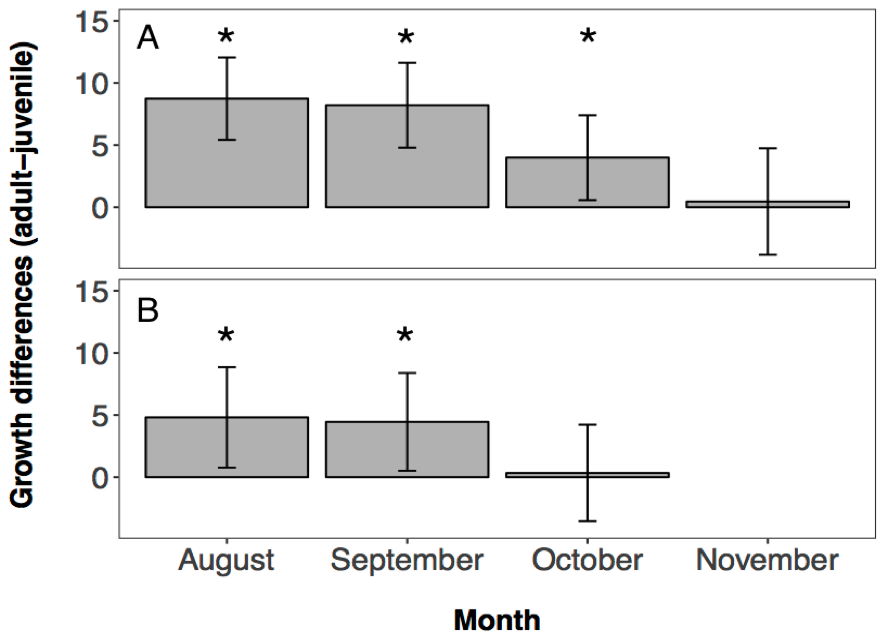
\includegraphics{images/data-chapter-3/growth-distributions.png}
\caption{\label{fig:growth-distributions}Estimates of otolith growth for
each juvenile cohort from (A) the Hutt River, and (B) the Wainuiomata
River ±95\% CI. Model calculates juvenile growth estimates relative to
the adult growth estimates. Therefore any estimate that is approximately
zero represents a juvenile otolith growth that is equal to the adult
otolith growth. Values above zero reflect faster juvenile growth
compared to adult survivor growth. Asterisks represent otolith growth
estimates significantly different from zero. No fishing was conducted in
the Wainuiomata River in November due to river mouth closure.}
\end{figure}

\section{Discussion}\label{discussion-2}

The main purpose of this chapter was to understand how hatch date and
growth history collectively shape survival in post-settlement fish.
Similarly to results from Chapter 2, each site exhibited different
patterns. In the Hutt River, hatch date distributions differed strongly
between adult fish and juvenile fish. However, in the Wainuiomata River,
there was no difference in hatch date distribution between life stages.
Adult populations from both rivers had relatively slow growth compared
to the juvenile fish. This slower growth also correlated with the growth
rate of juvenile fish entering the river in November (in the Hutt River)
and October (in the Wainuiomata River).

Shifts in hatch date distributions differed between each site. The
interpretation of this result is constrained by the mismatch in sampling
of adult G. maculatus between the two study sites, and the overall
limited sampling of adult fish. However, if the samples are an accurate
reflection of hatch date distributions, then the spatial differences
observed here could potentially be attributed either to different
post-settlement processes operating in each river, or it may be a
function of different phenotypic mixtures of juvenile fish entering each
river. Chapters 2 and 3 indicated that there were considerable
differences in the phenotypes of juvenile fish between each site.
Therefore, the input of phenotypically distinct cohorts into each river
may be responsible for the observed difference in adult composition.
Fish entering the Wainuiomata River were more phenotypically homogenous,
whereas fish entering the Hutt River were more phenotypically
heterogeneous (based on Chapter 2 results). If the Hutt River has a more
phenotypically diverse population of G. maculatus, then fitness linked
traits like hatch date and growth rate may have larger population level
effects, relative to a more homogenous population (McCauley et al.
1993). Juvenile fish entering the Hutt River may have spent time in
different environments and/or were from different natal sources. This
environmental heterogeneity may drive differences in growth rate, which
in turn affected their freshwater survival (Shima and Swearer 2010).
Therefore, post-settlement processes in each river may actually be
identical, but they produce different results in each river as they are
acting on the phenotypes of the G. maculatus population. This may have
interesting implications for my results from Chapter 3, as there I
suggested that mortality patterns were indiscriminate to phenotype.
Correlations between fitness and phenotypic traits may vary depending on
G. maculatus life stage, and therefore early life experiences may have
considerable flow on effects to later life stages (Meekan et al. 2010)

Fish from both rivers showed similar (but not identical) shifts in
growth rate distributions. My results suggest that adult fish had
comparatively slow otolith growth rates in their early life history.
Again, interpretation of these results is constrained by the limited
adult sampling. Shifts in the phenotypic distributions between juveniles
and adults may simply be the result of sample bias. However, if they are
an accurate reflection of traits at each life stage, then there are
several possibilities for these patterns. In many systems, growth rate
may be linked to fitness, and fish often experience selective mortality
on life history traits after settlement (Vigliola and Meekan 2002,
Raventós and Macpherson 2005, Vigliola et al. 2007, Shima and Swearer
2010). Predation has been shown to be an important source of
post-settlement mortality in other systems (Shulman 1985, Hixon 1991,
Connell 1996, Webster 2002), and is known to be a strong factor in
structuring freshwater fish communities (Goodgame and Miranda 1993,
Kohler et al. 1993, Jackson et al. 2001, Santucci Jr and Wahl 2003),
particularly when the predators are introduced species (Li and Moyle
1981). G. maculatus are preyed on by introduced trout (Crowl et al.
1992, Glova 2003, Bonnett and McIntosh 2004, Vigliano et al. 2009), and
this predation may be selective towards certain life history traits
(Werner and Hall 1974, Hambright 1991, Green and Côté 2014). Therefore,
a potential explanation for the shift in adult phenotypes towards slower
growth rates may be that selective mortality is operating on
post-settlement G. maculatus.

Adult fish in the Hutt River had significantly different hatch dates to
the juvenile fish hatch dates. A considerable body of literature has
indicated that hatch date can influence survival, with evidence that
either early (Confer and Cooley 1977, Houde 1989, Schupp 1990, Cargnelli
and Gross 1996), or late hatching (Garvey et al. 2002, Santucci Jr and
Wahl 2003, Kaemingk et al. 2013) can benefit survival. However, my
results indicate that an early vs late dichotomy may not be
representative for this species. Instead, fitness may be dependent upon
hatching at an `optimal' time that maximizes exposure to the best
environmental conditions, affording suitable growth rates for the next
life stage and environments. Hatching at the `wrong' time may result in
larvae having lower food availability (Cargnelli and Gross 1996), or
experiencing less favourable environmental conditions (Kramer and Smith
Jr 1962, Mooij et al. 1994). These conditions may influence phenotypic
variation (i.e.~alter growth rates), which may set them up better for
future success (Shima and Swearer 2010). Therefore, hatch date may not
directly influence freshwater survival, but it could expose fish to a
range of time- (or seasonally-) dependent conditions during their marine
dispersal phase.

While there is evidence that slow growth can be detrimental to young
fish (Crecco and Savoy 1985, Post and Prankevicius 1987, Danylchuk and
Tonn 2001, Vigliola et al. 2007), most of the support for the
`bigger-is-better' hypothesis comes from systems where predators become
gape-limited (Perez and Munch 2010). In systems where prey never outgrow
the gape of predators, fast growth may prove to be detrimental (Litvak
and Leggett 1992, Bertram and Leggett 1994). Larger fish are more likely
to be encountered, and attacked by predators (Fuiman 1989, Litvak and
Leggett 1992), whereas smaller fish can be more inconspicuous. Larger
fish are also known to feed in food rich microhabitats, which often
increases susceptibility and vulnerability to predators (Biro et al.
2006). Cushing (1990) suggested that the best survival came from fish
that could spend the least amount of time at a vulnerable size (i.e.,
the stage-duration hypothesis). However, it is unlikely that G.
maculatus ever reach a size where they are not vulnerable to predation
(Glova 2003), and therefore, remaining small and inconspicuous may offer
them the best chances for survival.

All fish that were older than 180 days had their growth profiles
truncated so that 180 was the maximum age observed. Otolith growth can
decouple from somatic growth post settlement (Hoey and McCormick 2004)
and I did not want this post-settlement growth to be considered by the
mixed effects model. 180 days was chosen as it was the approximate age
of the average juvenile fish, and therefore I considered it a good
approximation of the adult fish age at settlement. However, this
approach makes the assumption that the adult fish are part of the same
cohort as the juvenile fish, and indeed that using an `average age' is a
good way to estimate their pre-settlement growth. The missing link to
this puzzle lies in the adult fish age-at-settlement. A `settlement
mark' has been validated for G. maculatus (Hale and Swearer 2008),
however I was unable to locate a settlement mark in any of the adult
otoliths, and thus I was unable to estimate age-at-settlement. In
reality, adult survivors may be settling at a very different age to the
recruiting juvenile fish population and this `age effect' may be the
factor driving survivorship for certain individuals. As this data simply
isn't known, I believe that using an `average age' is an acceptable
method for analysis of growth histories. Future studies could use more
sophisticated techniques (i.e.~LA-ICPMS, as per Hale and Swearer 2008)
to consistently identify this settlement mark and confirm whether adult
fish are settling at similar ages.

Although the evidence presented in this chapter is circumstantial, it
has generated a novel hypothesis for the role of growth rate on
individual success in G. maculatus. Growth rate appears to be important
in freshwater populations of G. maculatus, however, results from Chapter
3 indicated that growth may not be tightly linked with fitness in marine
populations. This has implications for our understanding of the ecology
of G. maculatus, and suggests that fitness linked traits may change with
ontogeny. Hatch date may also have strong influences, as larval rearing
environment will likely shape juvenile growth rates. Future directions
should use experimental approaches to investigate predator-induced
selective mortality on G. maculatus (i.e.~through mesocosm approaches,
Parker 1971), and unravel the role of growth rate in both marine and
freshwater populations.

\chapter{Discussion}\label{discussion-3}

\section{Summary}\label{summary}

The primary aim of this thesis was to investigate how recruitment of the
amphidromous fish Galaxias maculatus varied across both spatial and
temporal scales, and the demographic consequences of this variation. New
Zealand has been a place of extensive research on G. maculatus, and
Galaxiids in general (Benzie 1968a, McDowall 1969, McDowall 1972,
McDowall et al. 1994, Hickford et al. 2010, Hickford and Schiel 2013).
Four of the five native Galaxiid species are currently threatened, and
this fishery is recognised as being socially, culturally, and
economically important to New Zealand (McDowall 1968, McDowall 1984,
Rowe et al. 1999). Therefore, studies pertaining to recruitment dynamics
of native Galaxiid fish are important for understanding how conservation
and management plans can be structured for the long term preservation of
these species.

This thesis concluded that 1) significant phenotypic variation can arise
in populations that recruit in close spatial (20 km) and temporal (one
day) proximity, 2) that mortality rates are, at best, weakly related to
larval quality, and 3) that adult freshwater populations of G. maculatus
may be partially shaped by growth rates experienced at sea, and hatch
dates. My results have revealed the importance of considering subtle
(and putatively minor) spatial and temporal differences in the context
of recruitment patterns, and ignoring these differences could lead to
poor interpretations and decisions. In addition, this work shows further
support for the idea that early life history can influence and predict
measures of adult survival. This thesis raises new questions, primarily
around the potential of local retention in harbour systems, the extent
to which recruitment can vary over seemingly small and insignificant
spatial and temporal scales, and of optimal growth strategies in the
post-settlement phase.

\section{Landscape features and dispersal
potential}\label{landscape-features-and-dispersal-potential}

Considerable research effort on G. maculatus has focussed on determining
the extent of natal homing (Barker and Lambert 1988, Waters et al. 2000,
Hickford and Schiel 2016), with recent genetic and otolith studies
suggesting that G. maculatus shows very little homing. Mitochondrial DNA
results from Waters et al (2000) suggests that G. maculatus show very
little population structure, due to the extent of gene flow during
marine dispersal. Similarly, otolith microchemistry results from
Hickford and Schiel (2016) suggest that less than three percent of
individuals return to their natal stream. However, there is also
evidence that G. maculatus larvae hatched on the east coast of New
Zealand will typically return to east coast rivers, and vice versa
(Hickford and Schiel 2016). Therefore, it seems unlikely that G.
maculatus larvae will regularly cross from the east to west coasts of
New Zealand, and there may be physical barriers (i.e.~water currents)
that prevent this level of dispersal (Chiswell and Rickard 2011).

Despite this apparent high level of larval mixing and low level of natal
return, one hypothesis I have proposed to explain my results throughout
this thesis is that the Hutt River shows an uncharacteristically high
level of philopatry, primarily due to the physical retentive properties
of the Wellington Harbour. There is extensive evidence that harbour
systems can promote retention of larvae by virtue of circulating
currents (Jessopp and McAllen 2007, Shima and Swearer 2009, Morgan et
al. 2011), and Wellington Harbour specifically has been suggested to
promote retention of fish larvae (Swearer and Shima 2010). Furthermore,
Wellington Harbour may act as a `nursery' ground, as it is nutrient
rich, supports high standing stocks of plankton (Helson et al. 2007),
and stays at optimal temperatures for G. maculatus growth (Maxwell 1956,
Mitchell 1989, Richardson et al. 1994). Nursery habitats are known to
retain and attract larvae (Caputi et al. 1996, Condie et al. 2011,
Beldade et al. 2016), and larvae are less likely to disperse far when
local conditions present a favourable and productive environment
(Swearer et al. 1999). Theoretically, Wellington Harbour appears to show
the characteristics of a retentive system, however this thesis has not
been a study of local retention and natal homing. While I can speculate
on the retentive properties of Wellington Harbour, this is a hypothesis
that needs to be empirically validated, and I discuss experimental
suggestions for this validation below.

\section{Variation in recruitment over spatial
scales}\label{variation-in-recruitment-over-spatial-scales}

The hypothesis of retention in harbour systems is closely linked with my
overall result that recruitment patterns vary over small spatial scales.
The explanations I have suggested above (i.e., water currents affecting
dispersal) may also play a strong role in driving the observed
difference between the juvenile fish entering the Hutt River compared to
the Wainuiomata River. The processes of recruitment are fundamentally
influenced by the availability of larvae (Gaines et al. 1985, Victor
1986, Milicich et al. 1992), and spatial variability in recruitment will
often arise from spatial differences in larval availability (Koslow et
al. 1987, Mann 1993). Larvae may drift passively with strong currents
(Williams et al. 1984, Cowen and Castro 1994, Weber et al. 2015), become
aggregated into higher densities by internal waves (Kingsford and Choat
1986, Shanks and Wright 1987, Greer et al. 2014), or be locally retained
by eddies (Mullaney and Suthers 2013, Beldade et al. 2016). Therefore,
these strong site-specific recruitment patterns may be driven by
different hydrodynamic processes acting on each river (Maxwell 1956,
Bowman et al. 1983). This has implications for studies of G. maculatus
recruitment, as it may prove difficult to make generalisations about
recruitment patterns without careful review of geographic position and
current influenced dispersal.

Spatial variation in phenotype patterns and larval retention can have
strong ecological consequences. Sites that have low levels of retention
may be considered demographically open, and become source populations
for other areas in a metapopulation (Jones et al. 2009). This is a
common pattern in amphidromous species due to their high dispersal
capabilities (McDowall 2007, McDowall 2010), but may lead to externally
regulated extinction balances. If a population does not self-recruit
then it is susceptible to high rates of local extinction due to
demographic stochasticity (Jones et al. 2009). However, other open
populations can then balance this local extinction through demographic
connectivity, and thus can show resilience over evolutionary time scales
(Kritzer and Sale 2006, McDowall 2010). Conversely, having high levels
of retention may lead to a population being demographically closed.
Closed populations can be regulated by either density-independent or
--dependent effects, which can have differing population consequences.
Closed populations regulated by density-dependent processes show low
susceptibility to local extinction and are able to persist through self
recruitment, yet have no way to be re-established following extinction
(Jones et al. 2009). Closed populations regulated by density-independent
processes have no internal regulation (Hixon et al. 2002), and therefore
are unlikely to recover following local extinction (Gonzalez et al.
1998, Hill et al. 2002). This metapopulation framework sets up an
interesting dynamic with the closely situated harbour-coast system.
Under the assumption that Wellington Harbour is a partially closed
population, and Cook Strait is primarily an open population, then the
persistence of the Wellington Harbour population may be dependent on how
much input it has from other systems. If Wellington Harbour was to
experience local extinction, then its recolonization may depend on
closely situated open populations like the Wainuiomata River.

\section{Effects of river mouth
closure}\label{effects-of-river-mouth-closure}

Migratory species can be classified as either obligate or facultative,
depending on whether their migration is a necessary step in completing
their life cycle (McDowall 1988, McDowall 1995). G. maculatus are
generally considered to be obligate migrants (McDowall 1995), despite
the presence of viable landlocked populations (Battini et al. 2000,
Barriga et al. 2002, Barriga et al. 2007). These landlocked populations
still undertake migrations, with newly hatched larvae moving from
spawning locations in streams to the limnetic zone of lakes (Pollard
1971). This obligatory migration can make amphidromous populations of G.
maculatus susceptible to the effects of river mouth closure. During
November 2015 the Wainuiomata River mouth was closed by gravel build-up,
and therefore juvenile G. maculatus were blocked from entering the
river. It is unknown whether closure of the Wainuiomata River mouth is a
common occurrence, but frequent closures may drive temporally variable
patterns in recruitment. My results from Chapter 2 showed that growth
rates decreased over the recruitment season, such that the Hutt River's
slowest growing monthly cohort of fish came from November. In Chapter 4,
I found that adult G. maculatus growth rates were overall very slow, and
that they matched juvenile growth rates from October in the Wainuiomata
River and November in the Hutt River. Chapter 4 also indicated that
there may be an `optimum' time to hatch, but this may not benefit
freshwater survival if fish are unable to enter the river. This may lead
to interesting metapopulation dynamics, where phenotypically `superior'
fish are unable to enter a freshwater habitat to settle. G. maculatus
juveniles may be forced to undertake further dispersal to find a new
river to enter. This may enhance demographic connectivity between
rivers, but may also increase temporal fluctuations in recruitment,
depending on the rivers susceptibility to closure (McDowall 1995).
Therefore, no fish entering the Wainuiomata River in November may have
affected patterns of adult recruitment, both in the Wainuiomata River
and geographically proximate rivers

\section{Future directions}\label{future-directions}

A central hypothesis I have proposed in this thesis is that Wellington
Harbour promotes a higher retention of larval G. maculatus (that likely
have hatched in the Hutt River) than would be expected in a coastally
positioned system. Waters et al (2000) used the mitochondrial CO1 gene
to conclude that there was no genetic population structure in New
Zealand. However the small number of migrants required to overcome
genetic differentiation may mask any evidence of short term isolation.
Therefore, a result of no population structure may be an artefact of a
small amount of mixing between harbour and coastal populations (Slatkin
1985). With this limitation, a more powerful approach may be to generate
whole genome data in the form of SNPs (single nucleotide polymorphisms).
Next generation techniques such as RAD sequencing (Baird et al. 2008)
and Genotyping-by-Sequencing (Elshire et al. 2011) would provide the
fine scale genetic data needed to detect whether harbour populations
experience higher retention of larval G. maculatus than typical coast
populations.

Results from Chapter 4 show that there was a correlation between
juveniles that had experienced slow marine growth during early life
stages, and the early life growth rate of adult fish. While there is
support in the literature for slow growth rates enhancing fitness
(Litvak and Leggett 1992), an experimental setup is required to
elucidate that slower growth rates are indeed a dominant factor in the
recruitment process for G. maculatus. Mesocosms have been successfully
used to test selective mortality on phenotypic traits (Parker 1971,
Hargreaves and LeBrasseur 1986, Caie 2016), and a similar approach may
be appropriate here, where a mesocosm is constructed that contains
juvenile G. maculatus and a natural predator (i.e., trout). A comparison
of the otoliths of consumed fish (from predator guts) and unconsumed
fish would facilitate conclusions about selective mortality on growth
rates, and whether slow growth is an optimum strategy for
post-settlement G. maculatus.

Chapters 2, 3, and 4 all made use of a dataset collected over a single
year of sampling. Although I was able to describe both spatial and
temporal patterns in my data, it is difficult to know whether these
patterns are consistent over multiple years. Similar studies by McDowall
(1994) and Barbee et al (2011) found results only weakly related to the
age and growth data presented in this thesis, which suggests that these
patterns might experience considerable annual fluctuations. Future
studies should try to accommodate multi-year sampling of juvenile and
adult G. maculatus in order to compare year-to-year phenotype
distributions and shifts.

\section{Conclusions}\label{conclusions}

In summary, populations of fish are comprised of individuals with
diverse early life histories and phenotypes. This diversity of life
histories can have implications for survival in both pre- and
post-settlement life stages, and is crucial for shaping the demographic
rates of populations. This thesis contributes to the knowledge that
early life history has carry over effects to future life stages, and
recruitment is dependent on smaller spatial and temporal scales than
previously thought. Therefore, context and life history should be
understood when describing the ecology of any organism, especially those
with stage structured life histories.

\chapter{References}\label{references}

Agrawal, A. A. (2001). ``Phenotypic plasticity in the interactions and
evolution of species.'' Science 294(5541): 321-326.

Amara, R., Y. Desaunay and F. Lagardere (1994). ``Seasonal variation in
growth of larval sole Solea solea (L.) and consequences on the success
of larval immigration.'' Netherlands Journal of Sea Research 32(3-4):
287-298.

Anderson, J. T. (1988). ``A review of size dependent survival during
pre-recruit stages of fishes in relation to recruitment.'' Journal of
Northwest Atlantic Fishery Science 8: 55-66.

Anderson, T. W. and D. A. Darling (1954). ``A test of goodness of fit.''
Journal of the American Statistical Association 49(268): 765-769.

Bagenal, T. (1971). ``The interrelation of the size of fish eggs, the
date of spawning and the production cycle.'' Journal of Fish Biology
3(2): 207-219.

Bailey, K. and E. Houde (1989). ``Predation on eggs and larvae of marine
fishes and the recruitment problem.'' Advances in marine biology 25:
1-83.

Bailey, K. M. (1994). ``Predation on juvenile flatfish and recruitment
variability.'' Netherlands Journal of Sea Research 32(2): 175-189.

Baird, N. A., P. D. Etter, T. S. Atwood, M. C. Currey, A. L. Shiver, Z.
A. Lewis, E. U. Selker, W. A. Cresko and E. A. Johnson (2008). ``Rapid
SNP discovery and genetic mapping using sequenced RAD markers.'' PLoS
One 3(10): e3376.

Baker, M. B. and S. Rao (2004). ``Incremental costs and benefits shape
natal dispersal: theory and example with Hemilepistus reaumuri.''
Ecology 85(4): 1039-1051.

Baker, T. T. and L. S. Timmons (1991). ``Precision of ages estimated
from five bony structures of Arctic char (Salvelinus alpinus) from the
Wood River System, Alaska.'' Canadian Journal of Fisheries and Aquatic
Sciences 48(6): 1007-1014.

Barbee, N. C., R. Hale, J. R. Morrongiello, A. S. Hicks, D. Semmens, B.
J. Downes and S. E. Swearer (2011). ``Large-scale variation in
life-history traits of the widespread diadromous fish, Galaxias
maculatus, reflects geographic differences in local environmental
conditions.'' Marine and Freshwater Research 62: 790-800.

Barker, J. R. and D. M. Lambert (1988). ``A genetic analysis of
populations of Galaxias maculatus from the Bay of Plenty: Implications
for natal river return.'' New Zealand Journal of Marine and Freshwater
Research 22(3): 321-326.

Barriga, J. P., M. A. Battini and V. E. Cussac (2007). ``Annual dynamics
variation of a landlocked Galaxias maculatus (Jenyns 1842) population in
a Northern Patagonian river: occurrence of juvenile upstream
migration.'' Journal of Applied Ichthyology 23(2): 128-135.

Barriga, J. P., M. A. Battini, M. García-Asorey, C. Carrea, P. J. Macchi
and V. E. Cussac (2012). ``Intraspecific variation in diet, growth, and
morphology of landlocked Galaxias maculatus during its larval period:
the role of food availability and predation risk.'' Hydrobiologia
679(1): 27-41.

Barriga, J. P., M. A. Battini, P. J. Macchi, D. Milano and V. E. Cussac
(2002). ``Spatial and temporal distribution of landlocked Galaxias
maculatus and Galaxias platei (Pisces : Galaxiidae) in a lake in the
South American Andes.'' New Zealand Journal of Marine and Freshwater
Research 36(2): 345-359.

Bastrikin, D. K., A. Gallego, C. P. Millar, I. G. Priede and E. G. Jones
(2014). ``Settlement length and temporal settlement patterns of juvenile
cod (Gadus morhua), haddock (Melanogrammus aeglefinus), and whiting
(Merlangius merlangus) in a northern North Sea coastal nursery area.''
ICES Journal of Marine Science: Journal du Conseil 71(8): 2101-2113.

Battini, M., V. Rocco, M. Lozada, B. Tartarotti and H. Zagarese (2000).
``Effects of ultraviolet radiation on the eggs of landlocked Galaxias
maculatus (Galaxiidae, Pisces) in northwestern Patagonia.'' Freshwater
Biology 44(3): 547-552.

Baumann, H. and M. Gagliano (2011). ``Changing otolith/fish size ratios
during settlement in two tropical damselfishes.'' Helgoland Marine
Research 65(3): 425.

Baumann, H., M. A. Peck and J.-P. Herrmann (2005). ``Short-term
decoupling of otolith and somatic growth induced by food level changes
in postlarval Baltic sprat, Sprattus sprattus.'' Marine and Freshwater
Research 56(5): 539-547.

Beldade, R., S. J. Holbrook, R. J. Schmitt, S. Planes and G. Bernardi
(2016). ``Spatial patterns of self‐recruitment of a coral reef fish in
relation to island‐scale retention mechanisms.'' Molecular Ecology
25(20): 5203-5211.

Benzie, V. (1968a). ``Some ecological aspects of the spawning behaviour
and early development of the common whitebait, Galaxias maculatus
attenuatus (Jenyns).'' Proceedings (New Zealand Ecological Society) 15:
31-39.

Bergenius, M. A., M. I. McCormick, M. G. Meekan and D. R. Robertson
(2005). ``Environmental influences on larval duration, growth and
magnitude of settlement of a coral reef fish.'' Marine Biology 147(2):
291-300.

Berra, T. M., L. Crowley, W. Ivantsoff and P. A. Fuerst (1996).
``Galaxias maculatus: an explanation of its biogeography.'' Marine and
Freshwater Research 47(6): 845-849.

Bertram, D. and W. Leggett (1994). ``Predation risk during the early
life history periods of fishes: separating the effects of size and
age.'' Marine Ecology Progress Series 109: 105-105.

Berven, K. A. (1990). ``Factors affecting population fluctuations in
larval and adult stages of the wood frog (Rana sylvatica).'' Ecology
71(4): 1599-1608.

Biro, P. A., M. V. Abrahams, J. R. Post and E. A. Parkinson (2004).
``Predators select against high growth rates and risk--taking behaviour
in domestic trout populations.'' Proceedings of the Royal Society of
London B: Biological Sciences 271(1554): 2233-2237.

Biro, P. A., M. V. Abrahams, J. R. Post and E. A. Parkinson (2006).
``Behavioural trade‐offs between growth and mortality explain evolution
of submaximal growth rates.'' Journal of Animal Ecology 75(5):
1165-1171.

Bjørnstad, O. N., J.-M. Fromentin, N. C. Stenseth and J. Gjøsæter
(1999). ``Cycles and trends in cod populations.'' Proceedings of the
National Academy of Sciences 96(9): 5066-5071.

Bogner, D. M., M. A. Kaemingk and M. R. Wuellner (2016). ``Consequences
of Hatch Phenology on Stages of Fish Recruitment.'' PLoS One 11(10):
e0164980.

Bolger, T. and P. Connolly (1989). ``The selection of suitable indices
for the measurement and analysis of fish condition.'' Journal of Fish
Biology 34(2): 171-182.

Bonnett, M. L. and A. R. McIntosh (2004). ``The influence of juvenile
brown trout (Salmo trutta) on habitat use of inanga (Galaxias maculatus)
in a stream simulator.'' Journal of the Royal Society of New Zealand
34(4): 357-367.

Bowman, M., A. Kibblewhite, R. Murtagh, S. Chiswell and B. Sanderson
(1983). ``Circulation and mixing in greater Cook Strait, New Zealand.''
Oceanologica acta 6(4): 383-391.

Brown, C. A. and S. H. Gruber (1988). ``Age assessment of the lemon
shark, Negaprion brevirostris, using tetracycline validated vertebral
centra.'' Copeia: 747-753.

Buijse, A. D. and R. P. Houthuijzen (1992). ``Piscivory, growth, and
size-selective mortality of age 0 pikeperch (Stizostedion lucioperca).''
Canadian Journal of Fisheries and Aquatic Sciences 49(5): 894-902.

Bunt, J. S. (1975). Primary productivity of marine ecosystems. Primary
productivity of the biosphere, Springer: 169-183.

Burgess, S. C. and D. J. Marshall (2011). ``Are numbers enough?
Colonizer phenotype and abundance interact to affect population
dynamics.'' Journal of Animal Ecology 80(3): 681-687.

Burgess, S. C., E. A. Treml and D. J. Marshall (2012). ``How do
dispersal costs and habitat selection influence realized population
connectivity?'' Ecology 93(6): 1378-1387.

Buston, P. M. and J. Elith (2011). ``Determinants of reproductive
success in dominant pairs of clownfish: a boosted regression tree
analysis.'' Journal of Animal Ecology 80(3): 528-538.

Caie, P. (2016). Selective mortality on early life-history traits of a
temperate reef fish (unpublished MSc thesis). Wellington, New Zealand,
Victoria University of Wellington.

Caley, M., M. Carr, M. Hixon, T. Hughes, G. Jones and B. Menge (1996).
``Recruitment and the local dynamics of open marine populations.''
Annual Review of Ecology and Systematics: 477-500.

Campana, S. E. and J. D. Neilson (1985). ``Microstructure of fish
otoliths.'' Canadian Journal of Fisheries and Aquatic Sciences 42(5):
1014-1032.

Cappo, M., P. Eden, S. J. Newman and S. Robertson (2000). ``A new
approach to validation of periodicity and timing of opaque zone
formation in the otoliths of eleven species of Lutjanus from the central
Great Barrier Reef.'' Fishery Bulletin 98(3): 474-474.

Caputi, N., W. Fletcher, A. Pearce and C. Chubb (1996). ``Effect of the
Leeuwin Current on the recruitment of fish and invertebrates along the
Western Australian coast.'' Marine and Freshwater Research 47(2):
147-155.

Cargnelli, L. M. and M. R. Gross (1996). ``The temporal dimension in
fish recruitment: birth date, body size, and size-dependent survival in
a sunfish (bluegill: Lepomis macrochirus).'' Canadian Journal of
Fisheries and Aquatic Sciences 53(2): 360-367.

Carrera, C., J. P. Barriga, V. E. Cussac and D. E. Ruzzante (2012).
``Genetic and phenotypic differentitation among Galaxias maculatus
populations in a Patagonian postglacial lake system.'' Biological
Journal of the Linnean Society 107: 368-382.

Cass, A. J. and R. J. Beamish (1983). ``First evidence of validity of
the fin-ray method of age determination for marine fishes.'' North
American Journal of Fisheries Management 3(2): 182-188.

Casselman, J. (1987). Determination of age and growth. The biology of
fish growth. S. Gill. London, Academic Press: 209-242.

Chambers, R. C. (1993). ``Phenotypic variability in fish populations and
its representation in individual-based models.'' Transactions of the
American Fisheries Society 122(3): 404-414.

Chambers, R. C. and W. C. Leggett (1987). ``Size and age at
metamorphosis in marine fishes: an analysis of laboratory-reared Winter
Flounder (Pseudopleutonectes americanus) with a review of variation in
other species.'' Canadian Journal of Fisheries and Aquatic Sciences
44(11): 1936-1947.

Chambers, R. C. and E. Trippel (2012). Early life history and
recruitment in fish populations, Springer Science \& Business Media.

Chapman, B. B., K. Hulthén, C. Brönmark, P. A. Nilsson, C. Skov, L. A.
Hansson and J. Brodersen (2015). ``Shape up or ship out: migratory
behaviour predicts morphology across spatial scale in a freshwater
fish.'' Journal of Animal Ecology 84: 1187-1193.

Chapman, D. and D. Robson (1960). ``The analysis of a catch curve.''
Biometrics: 354-368.

Chiswell, S. M. and G. J. Rickard (2011). ``Larval connectivity of
harbours via ocean currents: a New Zealand study.'' Continental Shelf
Research 31(10): 1057-1074.

Condie, S., J. Mansbridge and M. Cahill (2011). ``Contrasting local
retention and cross-shore transports of the East Australian Current and
the Leeuwin Current and their relative influences on the life histories
of small pelagic fishes.'' Deep Sea Research Part II: Topical Studies in
Oceanography 58(5): 606-615.

Confer, J. and J. Cooley (1977). ``Copepod instar survival and predation
by zooplankton.'' Journal of the Fisheries Board of Canada 34(5):
703-706.

Connell, S. (1996). ``Variations in mortality of a coral-reef fish:
links with predator abundance.'' Marine Biology 126(2): 347-352.

Conover, D. O. and E. T. Schultz (1997). ``Natural selection and the
evolution of growth rate in the early life history: what are the
trade-offs?'' Fish and Fisheries Series 21: 305-332.

Cowan, J. H., E. D. Houde and K. A. Rose (1996). ``Size-dependent
vulnerability of marine fish larvae to predation: an individual-based
numerical experiment.'' ICES Journal of Marine Science: Journal du
Conseil 53(1): 23-37.

Cowen, R. K. (2002). Larval dispersal and retention and consequences for
population connectivity. Coral reef fishes: New insights into their
ecology. P. F. Sale. London, Academic Press: 149-170.

Cowen, R. K. and L. R. Castro (1994). ``Relation of coral reef fish
larval distributions to island scale circulation around Barbados, West
Indies.'' Bulletin of Marine Science 54(1): 228-244.

Cowen, R. K. and S. Sponaugle (2009). ``Larval dispersal and marine
population connectivity.'' Annual Review Marine Science 1: 443-446.

Crean, A. J., K. Monro and D. J. Marshall (2011). ``Fitness consequences
of larval traits persist across the metamorphic boundary.'' Evolution
65(11): 3079-3089.

Crecco, V. A. and T. F. Savoy (1985). ``Effects of biotic and abiotic
factors on growth and relative survival of young American shad, Alosa
sapidissima, in the Connecticut River.'' Canadian Journal of Fisheries
and Aquatic Sciences 42(10): 1640-1648.

Crowl, T. A., C. R. Townsend and A. R. McIntosh (1992). ``The impact of
introduced brown and rainbow trout on native fish: the case of
Australasia.'' Reviews in Fish Biology and Fisheries 2(3): 217-241.

Cushing, D. (1969). ``The regularity of the spawning season of some
fishes.'' Journal du Conseil 33(1): 81-92.

Cushing, D. (1990). ``Plankton production and year-class strength in
fish populations: an update of the match/mismatch hypothesis.'' Advances
in marine biology 26: 249-293.

Cushing, D. H. (1975). Marine ecology and fisheries, CUP Archive.

Cussac, V., S. Ortubay, G. Iglesias, D. Milano, M. E. Lattuca, J. P.
Barriga, M. Battini and M. Gross (2004). ``The distribution of South
American galaxiid fishes: the role of biological traits and post-glacial
history.'' Journal of Biogeography 31(1): 103-121.

Cussac, V. E., P. M. Cervellini and M. Á. Battini (1992).
``Intralacustrine movements of Galaxias maculatus (Galaxiidae) and
Ondontesthes microlepidotus (Atherinidae) during their early life
history.'' Environmental Biology of Fishes 35: 141-148.

Dahlberg, M. D. (1979). ``A review of survival rates of fish eggs and
larvae in relation to impact assessments.'' Marine Fisheries Review
41(3): 1-12.

Danylchuk, A. J. and W. M. Tonn (2001). ``Effects of social structure on
reproductive activity in male fathead minnows (Pimephales promelas).''
Behavioral Ecology 12(4): 482-489.

Divino, J. and W. Tonn (2007). ``Effects of reproductive timing and
hatch date on fathead minnow recruitment.'' Ecology of Freshwater Fish
16(2): 165-176.

Dunn, A., R. Francis and I. Doonan (2002). ``Comparison of the
Chapman--Robson and regression estimators of Z from catch-curve data
when non-sampling stochastic error is present.'' Fisheries Research
59(1): 149-159.

Edeline, E. (2007). ``Adaptive phenotypic plasticity of eel diadromy.''
Marine Ecology Progress Series 341: 229-232.

Einum, S. (2003). ``Atlantic salmon growth in strongly food-limited
environments: Effects of egg size and paternal phenotype?''
Environmental Biology of Fishes 67(3): 263-268.

Elshire, R. J., J. C. Glaubitz, Q. Sun, J. A. Poland, K. Kawamoto, E. S.
Buckler and S. E. Mitchell (2011). ``A robust, simple
genotyping-by-sequencing (GBS) approach for high diversity species.''
PLoS One 6(5): e19379.

Essig, R. J. and C. F. Cole (1986). ``Methods of estimating larval fish
mortality from daily increments in otoliths.'' Transactions of the
American Fisheries Society 115(1): 34-40.

Fiksen, Ø., C. Jørgensen, T. Kristiansen, F. Vikebø and G. Huse (2007).
``Linking behavioural ecology and oceanography: larval behaviour
determines growth, mortality and dispersal.'' Marine Ecology Progress
Series 347: 195-205.

Fitzsimons, J. M., R. M. Zink and R. T. Nishimoto (1990). ``Genetic
variation in the Hawaiian stream goby, Lentipes concolor.'' Biochemical
Systematics and Ecology 18(1): 81-83.

Fogarty, M. J., M. P. Sissenwine and E. B. Cohen (1991). ``Recruitment
variability and the dynamics of exploited marine populations.'' Trends
in Ecology \& Evolution 6(8): 241-246.

Fouzai, N., A. F. Opdal, C. Jørgensen and Ø. Fiksen (2015). ``Effects of
temperature and food availability on larval cod survival: a model for
behaviour in vertical gradients.'' Marine Ecology Progress Series 529:
199-212.

Fowler, A. and P. Doherty (1992). ``Validation of annual growth
increments in the otoliths of two species of damselfish from the
southern Great Barrier Reef.'' Marine and Freshwater Research 43(5):
1057-1068.

Francis, M. P., M. W. Williams, A. C. Pryce, S. Pollard and S. G. Scott
(1993). ``Uncoupling of otolith and somatic growth in Pagrus auratus
(Sparidae).'' Fishery Bulletin - National Oceanic and Atmospheric
Administration 91: 159-164.

Fuiman, L. A. (1989). ``Vulnerability of Atlantic herring larvae to
predation by yearling herring.'' Marine Ecology Progress Series 51(3):
291-299.

Gagliano, M., M. I. McCormick and M. G. Meekan (2007). ``Survival
against the odds: ontogenetic changes in selective pressure mediate
growth-mortality trade-offs in a marine fish.'' Proceedings of the Royal
Society of London B: Biological Sciences 274(1618): 1575-1582.

Gaillard, J.-M., M. Festa-Bianchet, N. Yoccoz, A. Loison and C. Toigo
(2000). ``Temporal variation in fitness components and population
dynamics of large herbivores.'' Annual Review of Ecology and Systematics
31: 367-393.

Gaines, S., S. Brown and J. Roughgarden (1985). ``Spatial variation in
larval concentrations as a cause of spatial variation in settlement for
the barnacle, Balanus glandula.'' Oecologia 67(2): 267-272.

Gaines, S. D. and J. Roughgarden (1987). ``Fish in offshore kelp forests
affect recruitment to intertidal barnacle populations.'' Science
235(4787): 479-480.

Garvey, J. E., T. P. Herra and W. C. Leggett (2002). ``Protracted
reproduction in sunfish: the temporal dimesion in fish recruitment
revisited.'' Ecological Applications 12(1): 194-205.

GIMP Team (2016). GNU Image Manipulation Program.

Gleason, T. R. and D. A. Bengtson (1996). ``Size-selective mortality of
inland silversides: Evidence from otolith microstructure.'' Transactions
of the American Fisheries Society 125(6): 860-873.

Glova, G. (2003). ``A test for interaction between brown trout (Salmo
trutta) and inanga (Galaxias maculatus) in an artificial stream.''
Ecology of Freshwater Fish 12(4): 247-253.

Gonzalez, A., J. Lawton, F. Gilbert, T. Blackburn and I. Evans-Freke
(1998). ``Metapopulation dynamics, abundance, and distribution in a
microecosystem.'' Science 281(5385): 2045-2047.

Good, S., J. Dodson, M. Meekan and D. A. Ryan (2001). ``Annual variation
in size-selective mortality of Atlantic salmon (Salmo salar) fry.''
Canadian Journal of Fisheries and Aquatic Sciences 58(6): 1187-1195.

Goodgame, L. S. and L. E. Miranda (1993). ``Early growth and survival of
age-0 largemouth bass in relation to parental size and swim-up time.''
Transactions of the American Fisheries Society 122(1): 131-138.

Gosselin, L. A. and P.-Y. Qian (1997). ``Juvenile mortality in benthic
marine invertebrates.'' Marine Ecology Progress Series 146: 265-282.

Graham, W. M. and J. L. Largier (1997). ``Upwelling shadows as nearshore
retention sites: the example of northern Monterey Bay.'' Continental
Shelf Research 17(5): 509-532.

Green, B. S. and R. Fisher (2004). ``Temperature influences swimming
speed, growth and larval duration in coral reef fish larvae.'' Journal
of Experimental Marine Biology and Ecology 299(1): 115-132.

Green, S. J. and I. M. Côté (2014). ``Trait‐based diet selection: prey
behaviour and morphology predict vulnerability to predation in reef fish
communities.'' Journal of Animal Ecology 83(6): 1451-1460.

Greer, A. T., R. K. Cowen, C. M. Guigand, J. A. Hare and D. Tang (2014).
``The role of internal waves in larval fish interactions with potential
predators and prey.'' Progress in Oceanography 127: 47-61.

Grether, G. F. (2005). ``Environmental change, phenotypic plasticity,
and genetic compensation.'' The American Naturalist 166(4): E115-E123.

Grorud-Colvert, K. and S. Sponaugle (2006). ``Influence of condition on
behavior and survival potential of a newly settled coral reef fish, the
bluehead wrasse Thalassoma bifasciatum.'' Marine Ecology Progress Series
327: 279-288.

Grorud-Colvert, K. and S. Sponaugle (2011). ``Variability in water
temperature affects trait-mediated survival of a newly settled coral
reef fish.'' Oecologia 165(3): 675-686.

Gross, M. R., R. M. Coleman and R. M. McDowall (1988). ``Aquatic
productivity and the evolution of diadromous fish migration.'' Science
239(4845): 1291-1293.

Günther, C. C., J.-P. Herrmann and A. Temming (2015). ``Laboratory
calibration of optimal growth to deduce in situ feeding conditions of
early juvenile sprat Sprattus sprattus from otoliths.'' Marine Ecology
Progress Series 525: 199-215.

Hadfield, M. and M. Strathmann (1996). ``Variability, flexibility and
plasticity in life histories of marine invertebrates.'' Oceanologica
Acta 19(3-4): 323-334.

Hambright, K. D. (1991). ``Experimental analysis of prey selection by
largemouth bass: role of predator mouth width and prey body depth.''
Transactions of the American Fisheries Society 120(4): 500-508.

Hamilton, S. L. (2008). ``Larval history influences post-metamorphic
condition in a coral-reef fish.'' Oecologia 158(3): 449-461.

Hamilton, S. L., J. Regetz and R. R. Warner (2008). ``Postsettlement
survival linked to larval life in a marine fish.'' Proceedings of the
National Academy of Sciences 105(5): 1561-1566.

Handelsman, C. A., E. D. Broder, C. M. Dalton, E. W. Ruell, C. A.
Myrick, D. N. Reznick and C. K. Ghalambor (2013). ``Predator-induced
phenotypic plasticity in metabolism and rate of growth: rapid adaptation
to a novel environment.'' Integrative and Comparative Biology 53(6):
975-988.

Hargreaves, N. B. and R. J. LeBrasseur (1986). ``Size selectivity of
coho (Oncorhynchus kisutch) preying on juvenile chum salmon (O. keta).''
Canadian Journal of Fisheries and Aquatic Sciences 43(3): 581-586.

Harrod, C., J. Mallela and K. K. Kahilainen (2010).
``Phenotype‐environment correlations in a putative whitefish adaptive
radiation.'' Journal of Animal Ecology 79(5): 1057-1068.

Hartl, D. L. (1988). A primer of population genetics, Sinauer
Associates, Inc.

Helson, J. G., S. Pledger and J. P. Gardner (2007). ``Does differential
particulate food supply explain the presence of mussels in Wellington
Harbour (New Zealand) and their absence on neighbouring Cook Strait
shores?'' Estuarine, Coastal and Shelf Science 72(1): 223-234.

Hickford, M. J. and D. R. Schiel (2016). ``Otolith microchemistry of the
amphidromous Galaxias maculatus shows recruitment to coastal rivers from
unstructured larval pools.'' Marine Ecology Progress Series 548:
197-207.

Hickford, M. J. H., M. Cagnon and D. R. Schiel (2010). ``Predation,
vegetation and habitat-specific survival of terrestrial eggs of a
diadromous fish, Galaxias maculatus (Jenyns, 1842).'' Journal of
Experimental Marine Biology and Ecology 385(1-2): 66-72.

Hickford, M. J. H. and D. R. Schiel (2013). ``Artificial spawning
habitats improve egg production of a declining diadromous fish, galaxias
maculatus (Jenyns, 1842).'' Restoration Ecology 21(6): 686-694.

Hill, M. F., A. Hastings and L. W. Botsford (2002). ``The effects of
small dispersal rates on extinction times in structured metapopulation
models.'' The American Naturalist 160(3): 389-402.

Hixon, M. A. (1991). Predation as a process structuring coral reef fish
communities. The Ecology of Fishes on Coral Reefs. P. F. Sale. San
Diego, California, Academic Press: 475-508.

Hixon, M. A., S. W. Pacala and S. A. Sandin (2002). ``Population
regulation: historical context and contemporary challenges of open
vs.~closed systems.'' Ecology 83(6): 1490-1508.

Hjort, J. (1914). ``Fluctuations in the great fisheries of northern
Europe viewed in the light of biological research.'' Rapports et
Procès-Verbaux des Réunions du Conseil Permanent International Pour
L'Exploration de la Mer 20: 1-228.

Hoenig, J. M. (1983). ``Empirical use of longevity data to estimate
mortality rates.'' Fishery Bulletin 82(1): 898-903.

Hoey, A. S. and M. I. McCormick (2004). ``Selective predation for low
body condition at the larval-juvenile transition of a coral reef fish.''
Oecologia 139(1): 23-29.

Hoffnagle, T. L. and T. J. Timmons (1989). ``Age, growth, and catch
analysis of the commercially exploited paddlefish population in Kentucky
Lake, Kentucky-Tennessee.'' North American Journal of Fisheries
Management 9(3): 316-326.

Holmes, T. H. and M. I. McCormick (2006). ``Location influences
size-selective predation on newly settled reef fish.'' Marine Ecology
Progress Series 317: 203-209.

Houde, E. (1989). ``Subtleties and episodes in the early life of
fishes.'' Journal of Fish Biology 35: 29-38.

Houde, E. and R. Hoyt (1987). Fish early life dynamics and recruitment
variability. American Fisheries Science Symposium.

Houde, E. D. (1989). ``Comparative growth, mortality, and energetics of
marine fish larvae: Temperature and implied latitudinal effects.''
Fishery Bulletin 87(3): 471-495.

Houde, E. D. (1994). ``Differences between marine and freshwater fish
larvae - implications for recruitment.'' ICES Journal of Marine Science
51(1): 91-97.

Houde, E. D. (1997). ``Patterns and consequences of selective processes
in teleost early life histories.'' Fish and Fisheries Series 21:
173-196.

Houde, E. D. and C. E. Zastrow (1993). ``Ecosystem-and taxon-specific
dynamic and energetics properties of larval fish assemblages.'' Bulletin
of Marine Science 53(2): 290-335.

Hovenkamp, F. (1992). ``Growth-dependent mortality of larval plaice
Pleuronectes platessa in the North Sea.'' Marine Ecology Progress Series
82(1): 95-101.

Imre, I., R. McLaughlin and D. Noakes (2002). ``Phenotypic plasticity in
brook charr: changes in caudal fin induced by water flow.'' Journal of
Fish Biology 61(5): 1171-1181.

Irvine, R. L., D. C. Schmidt and L. R. Hildebrand (2007). ``Population
status of white sturgeon in the lower Columbia River within Canada.''
Transactions of the American Fisheries Society 136(6): 1472-1479.

Jackson, D. A., P. R. Peres-Neto and J. D. Olden (2001). ``What controls
who is where in freshwater fish communities the roles of biotic,
abiotic, and spatial factors.'' Canadian Journal of Fisheries and
Aquatic Sciences 58(1): 157-170.

Jacob, A., G. Evanno, E. Renai, R. Sermier and C. Wedekind (2009).
``Male body size and breeding tubercles are both linked to intrasexual
dominance and reproductive success in the minnow.'' Animal Behaviour
77(4): 823-829.

Jakob, E. M., S. D. Marshall and G. W. Uetz (1996). ``Estimating
fitness: a comparison of body condition indices.'' Oikos: 61-67.

Jellyman, P. G. and A. R. McIntosh (2008). ``The influence of habitat
availability and adult density on non-diadromous galaxiid fry settlement
in New Zealand.'' Journal of Fish Biology 72(1): 143-156.

Jenkins, G. P. and D. King (2006). ``Variation in larval growth can
predict the recruitment of a temperate, seagrass-associated fish.''
Oecologia 147(4): 641-649.

Jessopp, M. J. and R. J. McAllen (2007). ``Water retention and limited
larval dispersal: implications for short and long distance dispersers in
marine reserves.'' Marine Ecology Progress Series 333: 27-36.

Johnson, D. and M. Hixon (2010). ``Ontogenetic and spatial variation in
size‐selective mortality of a marine fish.'' Journal of Evolutionary
Biology 23(4): 724-737.

Johnson, D. W., K. Grorud‐Colvert, S. Sponaugle and B. X. Semmens
(2014). ``Phenotypic variation and selective mortality as major drivers
of recruitment variability in fishes.'' Ecology Letters 17(6): 743-755.

Johnston, I. A. (2006). ``Environment and plasticity of myogenesis in
teleost fish.'' Journal of Experimental Biology 209(12): 2249-2264.

Jones, G. (1986). ``Food availability affects growth in a coral reef
fish.'' Oecologia 70(1): 136-139.

Jones, G. P. (1990). ``The importance of recruitment to the dynamics of
a coral reef fish population.'' Ecology 71(5): 1691-1698.

Jones, G. P., G. R. Almany, G. Russ, P. Sale, R. Steneck, M. Van Oppen
and B. Willis (2009). ``Larval retention and connectivity among
populations of corals and reef fishes: history, advances and
challenges.'' Coral Reefs 28(2): 307-325.

Jones, G. P., S. Planes and S. R. Thorrold (2005). ``Coral reef fish
larvae settle close to home.'' Current Biology 15(14): 1314-1318.

Jonsson, B. (1985). ``Life history patterns of freshwater resident and
sea-run migrant brown trout in Norway.'' Transactions of the American
Fisheries Society 114(2): 182-194.

Kaemingk, M. A., K. J. Stahr, J. C. Jolley, R. S. Holland and D. W.
Willis (2013). ``Evidence for bluegill spawning plasticity obtained by
disentangling complex factors related to recruitment.'' Canadian Journal
of Fisheries and Aquatic Sciences 71(1): 93-105.

Kekalainen, J., J. Kahkonen, V. Kiviniemi and H. Huuskonen (2010).
``Morphological variation of perch Perca fluviatilis in humic lakes: the
effect of predator density, competition and prey abundance.'' Journal of
Fish Biology 76(4): 787-799.

Kell, L., S. Bonhommeau and J.-M. Fromentin (2013). ``A catch curve
analysis for east Atlantic and Mediterranean bluefin tuna.'' Collective
Volume of Scientific Papers 69(1): 199-203.

Kerr, L. A. and D. H. Secor (2009). ``Bioenergetic trajectories
underlying partial migration in Patuxent River (Chesapeake Bay) white
perch (Morone americana).'' Canadian Journal of Fisheries and Aquatic
Sciences 66(4): 602-612.

Kingsford, M. and J. Choat (1986). ``Influence of surface slicks on the
distribution and onshore movements of small fish.'' Marine Biology
91(2): 161-171.

Kohler, C. C., R. J. Sheehan and J. J. Sweatman (1993). ``Largemouth
bass hatching success and first-winter survival in two Illinois
reservoirs.'' North American Journal of Fisheries Management 13(1):
125-133.

Koslow, J. A., K. R. Thompson and W. Silvert (1987). ``Recruitment to
northwest Atlantic cod (Gadus morhua) and haddock (Melanogrammus
aeglefinus) stocks: influence of stock size and climate.'' Canadian
Journal of Fisheries and Aquatic Sciences 44(1): 26-39.

Kramer, R. H. and L. L. Smith Jr (1962). ``Formation of year classes in
largemouth bass.'' Transactions of the American Fisheries Society 91(1):
29-41.

Kritzer, J. P. and P. F. Sale (2006). The metapopulation ecology of
coral reef fishes. Marine metapopulations: 31-67.

Lande, R. and S. J. Arnold (1983). ``The measurement of selection on
correlated characters.'' Evolution 37(6): 1210-1226.

Langerhans, R. B., C. A. Layman, A. M. Shokrollahi and T. J. DeWitt
(2004). ``Predator-driven phenotypic diversification in Gambusia
affinis.'' Evolution 58(10): 2305-2318.

Largier, J. L. (2003). ``Considerations in estimating larval dispersal
distances from oceanographic data.'' Ecological Applications 13(1):
S71-S89.

Leggett, W. and E. Deblois (1994). ``Recruitment in marine fishes: is it
regulated by starvation and predation in the egg and larval stages?''
Netherlands Journal of Sea Research 32(2): 119-134.

Leis, J. M. (2006). ``Are Larvae of Demersal Fishes Plankton or
Nekton?'' Advances in marine biology 51: 57-141.

Lenth, R. V. (2016). ``Least-Squares Means: The R Package lsmeans.''
Journal of Statistical Software 69(1): 1-33.

Levin, L. A. (2006). ``Recent progress in understanding larval
dispersal: new directions and digressions.'' Integrative and Comparative
Biology 46(3): 282-297.

Li, H. W. and P. B. Moyle (1981). ``Ecological analysis of species
introductions into aquatic systems.'' Transactions of the American
Fisheries Society 110(6): 772-782.

Litvak, M. K. and W. C. Leggett (1992). ``Age and size-selective
predation on larval fishes: the bigger-is-better hypothesis revisited.''
Marine Ecology Progress Series 81(1): 13-24.

Losos, J. B., D. A. Creer, D. Glossip, R. Goellner, A. Hampton, G.
Roberts, N. Haskell, P. Taylor and J. Ettling (2000). ``Evolutionary
implications of phenotypic plasticity in the hindlimb of the lizard
Anolis sagrei.'' Evolution 54(1): 301-305.

MacDonald, B. and R. Thompson (1985). ``Influence of temperature and
food availability on the ecological energetics of the giant scallop
Placopecten magellanicus. I. Growth rates of shell and somatic tissue.''
Marine Ecology Progress Series 25(3): 279-294.

Mackas, D. L. and P. J. Harrison (1997). ``Nitrogenous nutrient sources
and sinks in the Juan de Fuca Strait/Strait of Georgia/Puget Sound
estuarine system: assessing the potential for eutrophication.''
Estuarine, Coastal and Shelf Science 44(1): 1-21.

Mann, K. (1993). ``Physical oceanography, food chains, and fish stocks:
a review.'' ICES Journal of Marine Science: Journal du Conseil 50(2):
105-119.

Maxwell, B. E. (1956). ``Hydrobiological observations for Wellington
Harbour.'' Transactions of the Royal Society of New Zealand 83(3):
493-503.

McCauley, E., W. G. Wilson and A. M. de Roos (1993). ``Dynamics of
age-structured and spatially structured predator-prey interactions:
individual-based models and population-level formulations.'' American
Naturalist 142(3): 412-442.

McCormick, M. I. (2006). ``Mothers matter: crowding leads to stressed
mothers and smaller offspring in marine fish.'' Ecology 87(5):
1104-1109.

McDowall, R. M. (1968). ``Galaxias maculatus (Jenyns) the New Zealand
whitebait.'' Fisheries Research Bulletin New Zealand No. 2: 1-84.

McDowall, R. M. (1969). ``Relationships of galaxioid fishes with a
further discussion of salmoniform classification.'' Copeia: 796-824.

McDowall, R. M. (1972). ``The species problem in freshwater fishes and
the taxonomy of diadromous and lacustrine populations of Galaxias
maculates (Jenyns).'' Journal of the Royal Society of New Zealand 2(3):
325-367.

McDowall, R. M. (1978). New Zealand freshwater fishes. Auckland,
Heinemann Educational.

McDowall, R. M. (1984). The New Zealand whitebait book. Wellington,
Reed.

McDowall, R. M. (1988). Diadromy in fishes: migrations between
freshwater and marine environments. London, Croom Helm.

McDowall, R. M. (1994). ``On size and growth in freshwater fish.''
Ecology of Freshwater Fish 3(2): 67-79.

McDowall, R. M. (1995). ``Seasonal pulses in migrations of New Zealand
diadromous fish and the potential impacts of river mouth closure.'' New
Zealand Journal of Marine and Freshwater Research 29(4): 517-526.

McDowall, R. M. (2002). ``Accumulating evidence for a dispersal
biogeography of southern cool temperate freshwater fishes.'' Journal of
Biogeography 29(2): 207-219.

McDowall, R. M. (2003). ``Hawaiian biogeography and the islands'
freshwater fish fauna.'' Journal of Biogeography 30(5): 703-710.

McDowall, R. M. (2007). ``On amphidromy, a distinct form of diadromy in
aquatic organisms.'' Fish and Fisheries 8: 1-13.

McDowall, R. M. (2009). ``Why be amphidromous: expatrial dispersal and
the place of source and sink population dynamics?'' Reviews in Fish
Biology and Fisheries 20(1): 87-100.

McDowall, R. M. (2010). ``Why be amphidromous: expatrial dispersal and
the place of source and sink population dynamics?'' Reviews in Fish
Biology and Fisheries 20(1): 87-100.

McDowall, R. M., D. Robertson and R. Saito (1975). ``Occurrence of
galaxiid larvae and juveniles in the sea.'' New Zealand Journal of
Marine and Freshwater Research 9(1): 1-9.

McDowall, R. M. and G. A. Eldon (1980). ``Ecology of whitebait
migrations (Galaxiidae: Galaxias spp).'' New Zealand Fisheries Research
Division Fisheries Research Bulletin(20): 1-171.

McDowall, R. M., C. P. Mitchell and E. B. Brothers (1994). ``Age at
migration from the sea of juvenile Galaxias in New Zealand (Pisces,
Galaxiidae).'' Bulletin of Marine Science 54(2): 385-402.

McDowall, R. M. and S. Charteris (2006). ``The possible adaptive
advantages of terrestrial egg deposition in some fluvial diadromous
galaxiid fishes (Teleostei: Galaxiidae).'' Fish and Fisheries 7(3):
153-164.

McGurk, M. D. (1986). ``Natural mortality of marine pelagic fish eggs
and larvae: role of spatial patchiness.'' Marine Ecology Progress Series
34(3): 227-242.

Media Cybernetics (2016). Image-Pro Premier. Rockville, Maryland, USA.

Meekan, M. and L. Fortier (1996). ``Selection for fast growth during the
larval life of Atlantic cod Gadus morhua on the Scotian Shelf.'' Marine
Ecology Progress Series 137: 25-37.

Meekan, M., J. Carleton, A. McKinnon, K. Flynn and M. Furnas (2003).
``What determines the growth of tropical reef fish larvae in the
plankton: food or temperature?'' Marine Ecology Progress Series 256:
193-204.

Meekan, M., L. Vigliola, A. Hansen, P. Doherty, A. Halford and J.
Carleton (2006). ``Bigger is better: size-selective mortality throughout
the life history of a fast-growing clupeid, Spratelloides gracilis.''
Marine Ecology Progress Series 317: 237-244.

Meekan, M. G., C. von Kuerthy, M. I. McCormick and B. Radford (2010).
``Behavioural mediation of the costs and benefits of fast growth in a
marine fish.'' Animal Behaviour 79(4): 803-809.

Milano, D., D. E. Ruzzante, V. E. Cussac, P. J. Macchi, R. A. Ferriz, J.
P. Barriga, J. C. Aigo, M. E. Lattuca and S. J. Walde (2006).
``Latitudinal and ecological correlates of morphological variation in
Galaxias platei (Pisces, Galaxiidae) in Patagonia.'' Biological Journal
of the Linnean Society 87: 69-82.

Milicich, M. M., M. M. Meekan and P. P. Doherty (1992). ``Larval supply:
a good predictor of recruitment of three species of reef fish
(Pomacentridae).'' Marine Ecology Progress Series 86: 153-166.

Miller, T. J., L. B. Crowder, J. A. Rice and E. A. Marschall (1988).
``Larval size and recruitment mechanisms in fishes: toward a conceptual
framework.'' Canadian Journal of Fisheries and Aquatic Sciences 45(9):
1657-1670.

Mitchell, C. P. (1989). ``Laboratory culture ofGalaxias maculatusand
potential applications.'' New Zealand Journal of Marine and Freshwater
Research 23(3): 325-336.

Moody, K., S. Hunter, M. Childress, R. Blob, H. Schoenfuss, M. Blum and
M. Ptacek (2015). ``Local adaptation despite high gene flow in the
waterfall‐climbing Hawaiian goby, Sicyopterus stimpsoni.'' Molecular
Ecology 24(3): 545-563.

Mooij, W., E. Lammens and W. V. Densen (1994). ``Growth rate of 0+ fish
in relation to temperature, body size, and food in shallow eutrophic
Lake Tjeukemeer.'' Canadian Journal of Fisheries and Aquatic Sciences
51(3): 516-526.

Morgan, S. G., J. L. Fisher and J. L. Largier (2011). ``Larval
retention, entrainment, and accumulation in the lee of a small headland:
Recruitment hotspots along windy coasts.'' Limnology and Oceanography
56(1): 161-178.

Mullaney, T. J. and I. M. Suthers (2013). ``Entrainment and retention of
the coastal larval fish assemblage by a short-lived, submesoscale,
frontal eddy of the East Australian Current.'' Limnology and
Oceanography 58(5): 1546-1556.

Munch, S. B., D. O. Conover and P. Wainwright (2003). ``Rapid growth
results in increased susceptibility to predation in Menidia menidia.''
Evolution 57(9): 2119-2127.

Murdoch, W. W. (1994). ``Population regulation in theory and practice.''
Ecology 75(2): 271-287.

Muylaert, K. and R. Raine (1999). ``Import, mortality and accumulation
of coastal phytoplankton in a partially mixed estuary (Kinsale harbour,
Ireland).'' Hydrobiologia 412: 53-65.

Myers, G. S. (1949). ``Usage of anadromous, catadromous and allied terms
for migratory fishes.'' Copeia: 89-97.

Myers, R., G. Mertz and J. Bridson (1997). ``Spatial scales of
interannual recruitment variations of marine, anadromous, and freshwater
fish.'' Canadian Journal of Fisheries and Aquatic Sciences 54(6):
1400-1407.

Newman, S. J., D. Williams and G. R. Russ (1996). ``Age validation,
growth and mortality rates of the tropical snappers (Pisces: Lutjanidae)
Lutjanus adetii (Castelnau, 1873) and L. quinquelineatus (Bloch, 1790)
from the central Great Barrier Reef, Australia.'' Marine and Freshwater
Research 47(4): 575-584.

Nicieza, A. G. and N. B. Metcalfe (1997). ``Growth compensation in
juvenile Atlantic salmon: responses to depressed temperature and food
availability.'' Ecology 78(8): 2385-2400.

Norris, D. R. (2005). ``Carry‐over effects and habitat quality in
migratory populations.'' Oikos 109(1): 178-186.

Ogle, D. H. (2016). FSA: Fisheries Stock Analysis.

Oliver, J. D., G. F. Holeton and K. E. Chua (1979). ``Overwinter
mortality of fingerling smallmouth bass in relation to size, relative
energy stores, and environmental temperature.'' Transactions of the
American Fisheries Society 108(2): 130-136.

Original S code by Richard A. Becker and Allan R. Wilks. R version by
Ray Brownrigg (2016). mapdata: Extra Map Databases.

Original S code by Richard A. Becker and Allan R. Wilks. R version by
Ray Brownrigg. Enhancements by Thomas P Minka and Alex Deckmyn (2016).
maps: Draw Geographical Maps.

Pannella, G. (1971). ``Fish otoliths - Daily growth layers and
periodical patterns.'' Science 173(4002): 1124-\&.

Parker, R. R. (1971). ``Size selective predation among juvenile salmonid
fishes in a British Columbia inlet.'' Journal of the Fisheries Board of
Canada 28(10): 1503-1510.

Pauly, D. (1990). ``Length-converted catch curves and the seasonal
growth of fishes.'' Fishbyte 8(3): 33-38.

Peel, R., G. Taylor and O. Weyl (2016). ``Validation of annulus
formation in sagittal otoliths of three tropical cichlids Oreochromis
andersonii (Castelnau, 1861), Oreochromis macrochir (Boulenger, 1912),
and Coptodon rendalli (Boulenger, 1896).'' Journal of Applied
Ichthyology 32: 859-865.

Pepin, P. (1987). ``Influence of alternative prey abundance on pelagic
fish predation of larval fish: a model.'' Canadian Journal of Fisheries
and Aquatic Sciences 44(1): 222-227.

Pepin, P. (1991). ``Effect of temperature and size on development,
mortality, and survival rates of the pelagic early life history stages
of marine fish.'' Canadian Journal of Fisheries and Aquatic Sciences
48(3): 503-518.

Pepin, P. (1992). ``Significance of body size to the interaction between
a larval fish (Mallotus villosus) and a vertebrate predator
(Gasterosteus aculeatus).'' Marine Ecology Progress Series 81: 1-12.

Perez, K. O. and S. B. Munch (2010). ``Extreme selection on size in the
early lives of fish.'' Evolution 64(8): 2450-2457.

Pfaff, M. C., G. M. Branch, J. L. Fisher, V. Hoffmann, A. G. Ellis and
J. L. Largier (2015). ``Delivery of marine larvae to shore requires
multiple sequential transport mechanisms.'' Ecology 96(5): 1399-1410.

Phillips, N. E. (2005). ``Growth of filter-feeding benthic invertebrates
from a region with variable upwelling intensity.'' Marine Ecology
Progress Series 295: 79-89.

Pineda, J., J. A. Hare and S. Sponaungle (2007). ``Larval transport and
dispersal in the coastal ocean and consequences for population
connectivity.'' Oceanography 20(3): 22-39.

Pineda, J., N. B. Reyns and V. R. Starczak (2009). ``Complexity and
simplification in understanding recruitment in benthic populations.''
Population ecology 51(1): 17-32.

Pinheiro, J., D. Bates, S. DebRoy, D. Sarkar and R Core Team (2016).
Linear and Nonlinear Mixed Effects Models.

Pollard, D. (1971). ``The biology of a landlocked form of the normally
catadromous salmoniform fish Galaxias maculatus (Jenyns). I. Life cycle
and origin.'' Marine and Freshwater Research 22(2): 91-124.

Post, J. R. and A. B. Prankevicius (1987). ``Size-selective mortality in
young-of-the-year yellow perch (Perca flavescens): evidence from otolith
microstructure.'' Canadian Journal of Fisheries and Aquatic Sciences
44(11): 1840-1847.

Radtke, R. L. and R. A. Kinzie (1996). ``Evidence of a marine larval
stage in endemic Hawaiian stream gobies from isolated high-elevation
locations.'' Transactions of the American Fisheries Society 125(4):
613-621.

Rätz, H.-J. and J. Lloret (2003). ``Variation in fish condition between
Atlantic cod (Gadus morhua) stocks, the effect on their productivity and
management implications.'' Fisheries Research 60(2): 369-380.

Raventós, N. and E. Macpherson (2005). ``Effect of pelagic larval growth
and size at hatching on the post-settlement survivorship in two
temperate labrid fishes of the genus Symphodus.'' Marine Ecology
Progress Series 285: 205-211.

Restrepo, V. R., J. Ortiz de Urbina, J.-M. Fromentin and H. Arrizabalaga
(2007). ``Estimates of selectivity for eastern Atlantic bluefin tuna
from catch curves.'' Collective Volume of Scientific Papers 60(3):
937-948.

Reznick, D. N. and C. K. Ghalambor (2001). ``The population ecology of
contemporary adaptations: what empirical studies reveal about the
conditions that promote adaptive evolution.'' Genetica 112(1): 183-198.

Richardson, J., J. A. Boubée and D. W. West (1994). ``Thermal tolerance
and preference of some native New Zealand freshwater fish.'' New Zealand
Journal of Marine and Freshwater Research 28(4): 399-407.

Ricker, W. E. (1975). Computation and interpretation of biological
statistics of fish populations, Dept. of Fisheries and Oceans.

Robillard, S. R. and J. E. Marsden (1996). ``Comparison of otolith and
scale ages for yellow perch from Lake Michigan.'' Journal of Great Lakes
Research 22(2): 429-435.

Robson, D. and D. Chapman (1961). ``Catch curves and mortality rates.''
Transactions of the American Fisheries Society 90(2): 181-189.

Rosenberg, A. and A. Haugen (1982). ``Individual growth and
size-selective mortality of larval turbot (Scophthalmus maximus) reared
in enclosures.'' Marine Biology 72(1): 73-77.

Roughgarden, J., S. Gaines and H. Possingham (1988). ``Recruitment
dynamics in complex life cycles.'' Science 241: 1460-1466.

Rowe, D. K., B. L. Chisnall, T. L. Dean and J. Richardson (1999).
``Effects of land use on native fish communities in east coast streams
of the North Island of New Zealand.'' New Zealand Journal of Marine and
Freshwater Research 33(1): 141-151.

RStudio Team (2015). RStudio: Integrated Development for R. Boston, MA,
RStudio Inc.

Rumrill, S. S. (1990). ``Natural mortality of marine invertebrate
larvae.'' Ophelia 32(1-2): 163-198.

Saccheri, I. and I. Hanski (2006). ``Natural selection and population
dynamics.'' Trends in Ecology \& Evolution 21(6): 341-347.

Sandström, O. and G. Thoresson (1988). ``Mortality in perch populations
in a Baltic pulp mill effluent area.'' Marine pollution bulletin 19(11):
564-567.

Santucci Jr, V. J. and D. H. Wahl (2003). ``The effects of growth,
predation, and first-winter mortality on recruitment of bluegill
cohorts.'' Transactions of the American Fisheries Society 132(2):
346-360.

Savino, J. F. and R. A. Stein (1989). ``Behavioural interactions between
fish predators and their prey: effects of plant density.'' Animal
Behaviour 37: 311-321.

Schluter, D., T. D. Price and L. Rowe (1991). ``Conflicting selection
pressures and life history trade-offs.'' Proceedings of the Royal
Society of London B: Biological Sciences 246(1315): 11-17.

Schneider, C. A., W. S. Rasband and K. W. Eliceiri (2012). ``NIH Image
to ImageJ: 25 years of image analysis.'' Nature methods 9(7): 671-675.

Schoener, T. W. (2011). ``The newest synthesis: understanding the
interplay of evolutionary and ecological dynamics.'' Science 331(6016):
426-429.

Scholz, F. W. and M. A. Stephens (1987). ``K-sample Anderson--Darling
tests.'' Journal of the American Statistical Association 82(399):
918-924.

Schupp, E. W. (1990). ``Annual variation in seedfall, postdispersal
predation, and recruitment of a neotropical tree.'' Ecology 71(2):
504-515.

Scott, D. E. (1994). ``The effect of larval density on adult demographic
traits in Ambystoma opacum.'' Ecology 75(5): 1383-1396.

Searcy, S. P. and S. Sponaugle (2000). ``Variable larval growth in a
coral reef fish.'' Marine Ecology Progress Series 206: 213-226.

Searcy, S. P. and S. Sponaugle (2001). ``Selective mortality during the
larval--juvenile transition in two coral reef fishes.'' Ecology 82(9):
2452-2470.

Shanks, A. L. and W. G. Wright (1987). ``Internal-wave-mediated
shoreward transport of cyprids, megalopae, and gammarids and correlated
longshore differences in the settling rate of intertidal barnacles.''
Journal of Experimental Marine Biology and Ecology 114(1): 1-13.

Shapiro, M. D., M. E. Marks, C. L. Peichel, B. K. Blackman, K. S.
Nereng, B. Jónsson, D. Schluter and D. M. Kingsley (2004). ``Genetic and
developmental basis of evolutionary pelvic reduction in threespine
sticklebacks.'' Nature 428(6984): 717-723.

Shepherd, J. and D. Cushing (1980). ``A mechanism for density-dependent
survival of larval fish as the basis of a stock-recruitment
relationship.'' Journal du Conseil 39(2): 160-167.

Shima, J. S. and A. M. Findlay (2002). ``Pelagic larval growth rate
impacts benthic settlement and survival of a temperate reef fish.''
Marine Ecology Progress Series 235: 303-309.

Shima, J. S. and S. E. Swearer (2009). ``Larval quality is shaped by
matrix effects: implications for connectivity in a marine
matapopulation.'' Ecology 90(5): 1255-1267.

Shima, J. S. and S. E. Swearer (2010). ``The legacy of dispersal: larval
experience shapes persistence later in the life of a reef fish.''
Journal of Animal Ecology 79(6): 1308-1314.

Shulman, M. J. (1985). ``Recruitment of coral reef fishes: effects of
distribution of predators and shelter.'' Ecology 66(3): 1056-1066.

Shuter, B., J. MacLean, F. Fry and H. Regier (1980). ``Stochastic
simulation of temperature effects on first-year survival of smallmouth
bass.'' Transactions of the American Fisheries Society 109(1): 1-34.

Siegel, D., B. Kinlan, B. Gaylord and S. Gaines (2003). ``Lagrangian
descriptions of marine larval dispersion.'' Marine Ecology Progress
Series 260: 83-96.

Simpson, A. C. (1959). ``The spawning of the plaice (Pleuronectes
platessa) in the North Sea.'' MAFF Fishery Investigations Series 2
22(7): 111.

Sissenwine, M. P. (1984). Why do fish populations vary? Exploitation of
marine communities. Berlin, Springer: 59-94.

Slatkin, M. (1985). ``Gene flow in natural populations.'' Annual Review
of Ecology and Systematics 16: 393-430.

Smith, D. C. (1987). ``Adult recruitment in chorus frogs: effects of
size and date at metamorphosis.'' Ecology 68(2): 344-350.

Smith, M. W., A. Y. Then, C. Wor, G. Ralph, K. H. Pollock and J. M.
Hoenig (2012). ``Recommendations for catch-curve analysis.'' North
American Journal of Fisheries Management 32(5): 956-967.

Soetaert, K. and P. M. Herman (1994). ``One foot in the grave:
zooplankton drift into the Westerschelde estuary (The Netherlands).''
Marine Ecology Progress Series 105(1-2): 19-29.

Sogard, S. M. (1997). ``Size-selective mortality in the juvenile stage
of teleost fishes: a review.'' Bulletin of Marine Science 60(3):
1129-1157.

Sorensen, M. C., J. M. Hipfner, T. K. Kyser and D. R. Norris (2009).
``Carry‐over effects in a Pacific seabird: stable isotope evidence that
pre‐breeding diet quality influences reproductive success.'' Journal of
Animal Ecology 78(2): 460-467.

Sponaugle, S., K. Grorud-Colvert and D. Pinkard (2006).
``Temperature-mediated variation in early life history traits and
recruitment success of the coral reef fish Thalassoma bifasciatum in the
Florida Keys.'' Marine Ecology Progress Series 308: 1-15.

Sponaugle, S., T. Lee, V. Kourafalou and D. Pinkard (2005). ``Florida
Current frontal eddies and the settlement of coral reef fishes.''
Limnology and Oceanography 50(4): 1033-1048.

Sponaugle, S. and D. Pinkard (2004). ``Impact of variable pelagic
environments on natural larval growth and recruitment of the reef fish
Thalassoma bifasciatum.'' Journal of Fish Biology 64(1): 34-54.

Staudinger, M. D. and F. Juanes (2010). ``Size-dependent susceptibility
of longfin inshore squid (Loligo pealeii) to attack and capture by two
predators.'' Journal of Experimental Marine Biology and Ecology 393(1):
106-113.

Stearns, S. C. (1992). The evolution of life histories, Oxford
University Press Oxford.

Stewart, B., G. Fenton, D. Smith and S. Short (1995). ``Validation of
otolith-increment age estimates for a deepwater fish species, the warty
oreo Allocyttus verrucosus, by radiometric analysis.'' Marine Biology
123(1): 29-38.

Sutherland, W. J., R. P. Freckleton, H. C. J. Godfray, S. R. Beissinger,
T. Benton, D. D. Cameron, Y. Carmel, D. A. Coomes, T. Coulson, M. C.
Emmerson, R. S. Hails, G. C. Hays, D. J. Hodgson, M. J. Hutchings, D.
Johnson, J. P. G. Jones, M. J. Keeling, H. Kokko, W. E. Kunin, X.
Lambin, O. T. Lewis, Y. Malhi, N. Mieszkowska, E. J. Milner-Gulland, K.
Norris, A. B. Phillimore, D. W. Purves, J. M. Reid, D. C. Reuman, K.
Thompson, J. M. J. Travis, L. A. Turnbull, D. A. Wardle and T. Wiegand
(2013). ``Identification of 100 fundamental ecological questions.''
Journal of Ecology 101(1): 58-67.

Svanback, R. and P. Eklov (2002). ``Effects of habitat and food
resources on morphology and ontogenetic growth trajectories in perch.''
Oecologia 131(1): 61-70.

Swearer, S. E., J. E. Caselle, D. W. Lea and R. R. Warner (1999).
``Larval retention and recruitment in an island population of a
coral-reef fish.'' Nature 402(6763): 799-802.

Swearer, S. E. and J. S. Shima (2010). ``Regional variation in larval
retention and dispersal drives recruitment patterns in a temperate reef
fish.'' Marine Ecology Progress Series 417: 229-236.

Swearer, S. E., J. S. Shima, M. E. Hellberg, S. R. Thorrold, G. P.
Jones, D. R. Robertson, S. G. Morgan, K. A. Selkoe, G. M. Ruiz and R. R.
Warner (2002). ``Evidence of self-recruitment in demersal marine
populations.'' Bulletin of Marine Science 70(1): 251-271.

Taubert, B. D. and D. W. Coble (1977). ``Daily rings in otoliths of
three species of Lepomis and Tilapia mossambica.'' Journal of the
Fisheries Board of Canada 34(3): 332-340.

Taylor, B. W., C. R. Anderson and B. L. Peckarsky (1998). ``Effects of
size at metamorphosis on stonefly fecundity, longevity, and reproductive
success.'' Oecologia 114(4): 494-502.

Taylor, G. C., R. A. Peel, C. J. Hay and O. L. Weyl (2016). ``Validation
of the periodicity of growth zone formation in the otoliths of four fish
species from the Upper Zambezi ecoregion, southern Africa.'' African
Zoology 51(3): 1-7.

Thorson, G. (1950). ``Reproductive and larval ecology of marine bottom
invertebrates.'' Biological reviews 25(1): 1-45.

Tonn, W. M. and C. A. Paszkowski (1986). ``Size-limited predation,
winterkill, and the organization of Umbra-Perca fish assemblages.''
Canadian Journal of Fisheries and Aquatic Sciences 43(1): 194-202.

Trussell, G. C. and L. D. Smith (2000). ``Induced defenses in response
to an invading crab predator: An explanation of historical and
geographic phenotypic change.'' Proceedings of the National Academy of
Sciences of the United States of America 97(5): 2123-2127.

Tsukamoto, K., H. Kuwada, J. Hirokawa, M. Oya, S. Sekiya and H. Fujimoto
(1989). ``Size‐dependent mortality of red sea bream, Pagrus major,
juveniles released with fluorescent otolith‐tags in News Bay, Japan.''
Journal of Fish Biology 35(sA): 59-69.

Victor, B. (1982). ``Daily otolith increments and recruitment in two
coral-reef wrasses, Thalassoma bifasciatum and Halichoeres bivittatus.''
Marine Biology 71(2): 203-208.

Victor, B. C. (1986). ``Larval settlement and juvenile mortality in a
recruitment‐limited coral reef fish population.'' Ecological Monographs
56(2): 145-160.

Vigliano, P. H., D. A. Beauchamp, D. Milano, P. J. Macchi, M. F. Alonso,
M. I. G. Asorey, M. A. Denegri, J. E. Ciancio, G. Lippolt and M.
Rechencq (2009). ``Quantifying predation on galaxiids and other native
organisms by introduced rainbow trout in an ultraoligotrophic lake in
northern Patagonia, Argentina: a bioenergetics modeling approach.''
Transactions of the American Fisheries Society 138(6): 1405-1419.

Vigliola, L. (1997). ``Validation of daily increment formation in
otoliths for three Diplodus species in the Mediterranean sea.'' Journal
of Fish Biology 51(2): 349-360.

Vigliola, L., P. J. Doherty, M. G. Meekan, D. M. Drown, M. E. Jones and
P. H. Barber (2007). ``Genetic identity determines risk of
post-settlement mortality of a marine fish.'' Ecology 88(5): 1263-1277.

Vigliola, L. and M. G. Meekan (2002). ``Size at hatching and planktonic
growth determine post-settlement survivorship of a coral reef fish.''
Oecologia 131(1): 89-93.

Vilizzi, L. and G. H. Copp (2013). ``Bias, precision and validation of
ageing 0+ European barbel Barbus barbus (L.) from their otoliths.''
Central European Journal of Biology 8(7): 654-661.

Ward, B. and P. Slaney (1988). ``Life history and smolt-to-adult
survival of Keogh River steelhead trout (Salmo gairdneri) and the
relationship to smolt size.'' Canadian Journal of Fisheries and Aquatic
Sciences 45(7): 1110-1122.

Ware, D. (1975). ``Relation between egg size, growth, and natural
mortality of larval fish.'' Journal of the Fisheries Board of Canada
32(12): 2503-2512.

Waters, J. M. and C. P. Burridge (1999). ``Extreme Intraspecific
Mitochondrial DNA Sequence Divergence inGalaxias maculatus (Osteichthys:
Galaxiidae), One of the World's Most Widespread Freshwater Fish.''
Molecular Phylogenetics and Evolution 11(1): 1-12.

Waters, J. M., L. H. Dijkstra and G. P. Wallis (2000). ``Biogeography of
a southern hemisphere freshwater fish: how important is marine
dispersal?'' Molecular Ecology 9(11): 1815-1821.

Weber, E. D., Y. Chao, F. Chai and S. McClatchie (2015). ``Transport
patterns of Pacific sardine Sardinops sagax eggs and larvae in the
California Current System.'' Deep Sea Research Part I: Oceanographic
Research Papers 100: 127-139.

Webster, M. S. (2002). ``Role of predators in the early post-settlement
demography of coral-reef fishes.'' Oecologia 131(1): 52-60.

Werner, E. E. and D. J. Hall (1974). ``Optimal foraging and the size
selection of prey by the bluegill sunfish (Lepomis macrochirus).''
Ecology 55(5): 1042-1052.

Werner, E. E., D. J. Hall, D. R. Laughlin, D. J. Wagner, L. A. Wilsmann
and F. C. Funk (1977). ``Habitat partitioning in a freshwater fish
community.'' Journal of the Fisheries Board of Canada 34(3): 360-370.

White, J. W., S. G. Morgan and J. L. Fisher (2014). ``Planktonic larval
mortality rates are lower than widely expected.'' Ecology 95(12):
3344-3353.

Williams, D. M., E. Wolanski and J. Andrews (1984). ``Transport
mechanisms and the potential movement of planktonic larvae in the
central region of the Great Barrier Reef.'' Coral Reefs 3(4): 229-236.

Wilson, D. T. and M. I. McCormick (1997). ``Spatial and temporal
validation of settlement-marks in the otoliths of tropical reef
fishes.'' Marine Ecology Progress Series 153: 259-271.

Windsland, K. (2014). ``Total and natural mortality of red king crab
(Paralithodes camtschaticus) in Norwegian waters: catch--curve analysis
and indirect estimation methods.'' ICES Journal of Marine Science:
Journal du Conseil fsu138: 1-19.

Woodson, C. and M. McManus (2007). ``Foraging behavior can influence
dispersal of marine organisms.'' Limnology and Oceanography 52(6):
2701-2709.

\bibliography{book.bib,packages.bib}

\end{document}
